\documentclass[11pt]{amsart}
% \documentclass[11pt]{article}
\linespread{1.25}

%%%%%%%%%%%%%%%%%%% P A C K A G E S %%%%%%%%%%%%%%%%%%%
\usepackage[margin=.8in]{geometry}
\usepackage{amsthm}
\usepackage{amsmath}
\usepackage{amssymb}
\usepackage{mathrsfs}
\usepackage{amsfonts}
\usepackage{graphicx}
\usepackage{pgf,tikz}
\usepackage{xcolor}
\usepackage{enumerate}
\usepackage{multicol}
\usepackage{graphpap}
\usepackage{parskip}
\usepackage{pgfplots}
\pgfplotsset{compat = newest}
% \usepackage[right]{showlabels}
\usepackage{xpatch}
\makeatletter
\xpatchcmd{\@thm}{\thm@headpunct{.}}{\thm@headpunct{}}{}{}
\makeatother
\pagestyle{headings}
%%%%%%%%%%%%%%%%%%% P A C K A G E S %%%%%%%%%%%%%%%%%%%



%%%%%%%%%%%%%%%%%%% E N V I R O N M E N T S %%%%%%%%%%%%%%%%%%%
\theoremstyle{plain}
\newtheorem{theorem}{Theorem}[section]
\newtheorem{proposition}[theorem]{Proposition} 
\newtheorem{lemma}[theorem]{Lemma}
\newtheorem{sublemma}[theorem]{Sublemma}
\newtheorem{corollary}[theorem]{Corollary}
\newtheorem{conjecture}[theorem]{Conjecture}
\newtheorem{exercise}[theorem]{Exercise}
\newtheorem{eg}[theorem]{Example}
\newtheorem{fig}{Figure} [section]
\theoremstyle{definition}
\newtheorem{definition}[theorem]{Definition}
\newtheorem{remark}[theorem]{Remark}
\newtheorem{question}[theorem]{Question}
\newtheorem{problem}[theorem]{Problem}
%%%%%%%%%%%%%%%%%%% E N V I R O N M E N T S %%%%%%%%%%%%%%%%%%%



%%%%%%%%%%%%%%%%%%% C O M M A N D S %%%%%%%%%%%%%%%%%%%
\newcommand{\N}{\mathbb N}
\newcommand{\R}{\mathbb R}
\newcommand{\Z}{\mathbb Z}
\newcommand{\Q}{\mathbb{Q}}
\newcommand{\C}{\mathbb{C}}
\newcommand{\UP}{\upharpoonright}
%%%%%%%%%%%%%%%%%%% C O M M A N D S %%%%%%%%%%%%%%%%%%%


\begin{document}
\title{\vspace{-5ex}\textbf{The Fourier Series \& its Applications}}
\author{\textbf{Claire Gillaspy \& Justin Hager}\\MTH 450: Real Analysis -- Fall 2022\\Furman University}
\date{}

\maketitle
\thispagestyle{empty}
% \tableofcontents
% \newpage
\section{Introduction}
The Fourier Series is one of the most utilized mathematical algorithms in modern technology. But, its roots date further back than the days of media compression, its primary application today. In 1822, Mathematician Joseph Fourier boldly stated ``there is no function $f$, or part of a function, which cannot be expressed by a trigonometric series" \cite{Fourier}. The work that led to this monumental advancement of mathematics was inspired by d'Alembret's use of trigonometric solutions to partial differential equations. In the book \textit{Understanding Analysis}, Abbott asserts the significance of Fourier's discovery, saying ``it is difficult to exaggerate the mathematical richness of this idea" \cite{Abbott}. 

Jean Baptist Joseph Fourier (1768 - 1830) was a French mathematician who was taught notably by Lagrange and Laplace. He studied the propagation of heat and solved the partial differential equation governing heat diffusion using infinite series of trigonometric functions. He had close relations with Napoleon and even worked as scientific adviser for Napoleon's army. He was a lifelong academic and continued to publish papers until his death at age 62, when he fell down the stairs in his own home \cite{Biography}.

In this paper, we outline the motivations behind the Fourier Series, its derivation, as well as various examples and applications of its utility. To preface, we introduce d'Alembret's wave equation and its connections to trigonometric series. Then, after outlining some foundational properties of trigonometric integration, we introduce the Fourier Transform and its derivations. Following two unique examples of the Fourier Series representation, we highlight its key features of continuity and infinite differentiability. Lastly, we introduce applications of the Discrete and Fast Fourier Transforms.

\section{Building the Base}
Before we introduce the Fourier Transform and its derivations, we must set the mathematical stage for the context in which Joseph Fourier published his work and acknowledge some of the trigonometric integral proprieties that will be crucial for the derivations to follow. 

\subsection{The Vibrating String Model}
Around 50 years prior to Fourier's work, Jean Le Rond d'Alembret (1717--1783) began the conversation of trigonometric approximation through his model of a vibrating string between two fixed endpoints. In this model, the function $u(x,t)$ represents the position of the string at any given point $x$ and time $t\geq 0$ \cite{Abbott}. Assuming the string covers the interval $[0,\pi]$, d'Alembret concluded that
\begin{equation}\label{eq:string1}
    u(0,t) = u(\pi,t) = 0.
\end{equation}
Further, given any initial displacement, he noted that the strings velocity at $t=0$ would satisfy
\begin{equation}\label{eq:string2}
    \dfrac{\partial u}{\partial t}(x,0) = 0.
\end{equation}
Lastly, he proposed that the second partial derivatives in respect to $x$ and $t$ would be equal, 
\begin{equation} \label{eq:string3}
    \frac{\partial^2 u}{\partial x^2}= \frac{\partial^2 u}{\partial t^t}.
\end{equation}
From Equations \ref{eq:string1}, \ref{eq:string2}, and \ref{eq:string3}, d'Alembret proposed the following theorem in search of a function to solve his so called `wave equation' \cite{Abbott}.

\begin{theorem}
    Any function of the form \[u(x,t)=\sum_{n=1}^N b_n\sin(nx)\cos(nt)\] where $N\in\N$ and $b_n\in \R $ satisfies d'Alembret's wave equation. 
\end{theorem}
If we consider only the case when $t=0$, then d'Alembret's wave equation has the capability to model the starting position of any `plucked' string. From this notion, Daniel Bernoulli proposed that any function $f$ could be thought of as the string's `starting position' and thus be modeled by the infinite trigonometric series \cite{Abbott}. The monumental work of both d'Alembret and Bernoulli is eventually what lead Joseph Fourier to his conclusions published in \textit{Théorie Analytique de la Chaleur} (The Analytical Theory of Heat, 1822) \cite{Fourier}.


\subsection{Trigonometric Integral Properties}
Before embarking upon the derivation of the Fourier Series, we must first establish some necessary components from calculus. Each part of the following example proves to be helpful in the work that is to come. 
\begin{eg}[\cite{Abbott}] \label{trig} %Exercise 8.5.2
    Let $L\in\R$ and verify the following properties of trigonometric integration
    \begin{enumerate}[(i)]
        \item For all $n\in \N$, $\int_{-L}^{L} \cos(nx)dx =0$ and $\int_{-L}^{L} \sin(nx)dx =0$ \label{trig1}
        \item For all $n\in \N$, $\int_{-L}^{L} \cos^2(nx)dx = L$ and $\int_{-L}^{L} \sin^2(nx)dx = L$ \label{trig2}
        \item For all $n,m\in \N$, $\int_{-L}^{L} \sin(nx)\cos(mx)dx =0$ \label{trig3}
        \item For all $n\neq m\in \N$, $\int_{-L}^{L} \cos(mx)\cos(nx)dx =0$ and $\int_{-L}^{L} \sin(mx)\sin(nx)dx =0$ \label{trig4}
    \end{enumerate}
\end{eg}
\begin{proof} Use calculus to verify,
    \begin{enumerate}[(i)]
    \setlength\itemsep{1em}
        \item For all $n\in \N$, \begin{align*}
            \int_{-L}^L \cos(nx)dx &= \frac{1}{n}(\sin(nL)-\sin(-nL)) = 0 \\
            \int_{-L}^L \sin(nx)dx &= \frac{-1}{n}(\cos(nL)-\cos(-nL)) = 0 \end{align*}
        \item For all $n\in \N$, \\
        \begin{minipage}{0.5\textwidth}
            \begin{align*}
                \int_{-L}^L \cos^2(nx)dx &= \frac{1}{2}\int_{-L}^L 1+ \cos(2nx)dx \\
                &= \frac{1}{2} \left[ L -(-L) \right] = L,
            \end{align*}
        \end{minipage}
        \begin{minipage}{0.5\textwidth}
        \begin{align*}
            \int_{-L}^L \sin^2(nx)dx &= \frac{1}{2}\int_{-L}^L 1- \cos(2nx)dx \\
            &= \frac{1}{2} \left[ L -(-L) \right] = L.
        \end{align*}
        \end{minipage}[t]
        \item For all $n,m \in \N$,
        \begin{align*}
            \int_{-L}^{L} \sin(nx)\cos(mx)dx &= \int_{-L}^{L} \dfrac{\sin((n+m)x)}{2} + \dfrac{\sin((n-m)x)}{2}dx\\
            &= \left[\dfrac{-1}{2(n+m)}cos((n+m)x)-\dfrac{1}{2(n-m)}cos((n-m)x)\right]_{-L}^L\\
            &= \left[\dfrac{-1}{2(n+m)}cos((n+m)L)-\dfrac{1}{2(n-m)}cos((n-m)L)\right]\\
            &\ -\left[\dfrac{-1}{2(n+m)}cos(-(n+m)L)-\dfrac{1}{2(n-m)}cos(-(n-m)L)\right]\\
            &= 0.
        \end{align*}
        \item A similar process as (\ref{trig3}), shows that for all $n\neq m\in \N$, it follows that, $$\int_{-L}^{L} \cos(mx)\cos(nx)dx =\int_{-L}^{L} \sin(mx)\sin(nx)dx  = 0.$$
    \end{enumerate}
\end{proof}
In addition to the above properties of trigonometric integration, we consider the two following lemmas. 
\begin{lemma} \label{lem:trig1}
    For any $n\in\N$, $cos(n\pi) = (-1)^n$.
\end{lemma}
\vspace{-0.5cm}
\begin{proof}
    Cosine is a periodic function with a period $2\pi$ where $\cos(\pi) = -1$ and $\cos(2\pi)= 1$. Further, if $n \in \N$ is even, $\cos(n\pi)= 1$ and if $n \in \N$ is odd, $\cos(n\pi) = -1.$ Thus, $\cos(n\pi) = (-1)^n$ for all $n\in\N.$
\end{proof}

\begin{lemma} \label{lem:trig2}
    For any $n\in\N$, $sin(n\pi) = 0$.
\end{lemma}
\vspace{-0.5cm}
\begin{proof}
    Sine is also a periodic function with a period of $2\pi$, but at every interval of $\pi$, $\sin(x)$ crosses the $x$-axis and $\sin(x)=0$. Thus, $\sin(n\pi) = 0$ for any $n\in N$ and $n=0$. 
\end{proof}

\section{Derivations}
\subsection{Deriving the Fourier Coefficients}\label{deriving}
As mentioned in the introduction, Fourier built from the work of d'Alemebret and the solution to his wave equation to conclude that any function $f$ could be accurately represented by an infinite trigonometric series.

\begin{theorem}
    Let $f:[-\pi,\pi]\to\R$ be an arbitrary function. If $f$ can be expressed as an infinite trigonometric series in the form 
    \begin{equation}
        \label{eqn:fourier}
        f(x) = a_0 + \sum_{n=1}^\infty a_n\cos(nx) + b_n\sin(nx),
        \end{equation}
    then the coefficients  $a_0$, $a_n$, and $b_n$ are given by
    \begin{enumerate}[(i)]
        \item $a_0=\dfrac{1}{2\pi}\int_{-\pi}^{\pi}f(x)dx$,
        \item $a_n=\int_{-\pi}^{\pi}f(x)\cos(\pi nx)dx$,
        \item $b_n=\int_{-\pi}^{\pi}f(x)\sin(\pi nx)dx.$
    \end{enumerate}
\end{theorem}
\begin{proof}
	Let $f$ be an arbitrary function for which can be represented as infinite trigonometric series. 
    \begin{enumerate}[(i)]
    \item Consider Equation \ref{eqn:fourier} and integrate both sides over $[-\pi, \pi]$. As a result, we have
    \begin{align*}
        \int_{-\pi}^{\pi} f(x) dx &= \int_{-\pi}^{\pi} \left[ a_0 + \sum_{n=1}^\infty a_n\cos(nx) + b_n\sin(nx)\right]dx\\
        &= \int_{-\pi}^{\pi}a_0 dx + \int_{-\pi}^{\pi} \left[\sum_{n=1}^\infty a_n\cos(nx) + b_n\sin(nx)\right]dx\\
        &= 2\pi a_0 + \int_{-\pi}^{\pi} \left[\sum_{n=1}^\infty a_n\cos(nx) + b_n\sin(nx)\right]dx.
    \end{align*}
    We are now faced with integrating an infinite series of trigonometric functions. From Theorem 7.4.2 (i) \cite{Abbott}, we integrate each term of the series individually, then apply the summation to the series of anti-derivatives. Using this method, we have that
    \begin{align*}
        \int_{-\pi}^{\pi} f(x) dx &= 2\pi a_0 + \sum_{n=1}^\infty\left[\int_{-\pi}^{\pi}\left(a_n\cos (nx) + b_n\sin(nx)\right)dx\right]\\
        &= 2\pi a_0 + \sum_{n=1}^\infty\left[a_n\int_{-\pi}^{\pi}\cos (nx)dx + b_n\int_{-\pi}^{\pi}\sin(nx)dx\right](\dagger)\\
        &= 2\pi a_0 + \sum_{n=1}^\infty a_n\cdot0 + b_n\cdot0\\
        &= 2\pi a_0,
    \end{align*}
    where $(\dagger)$ was computed using Example \ref{trig} (\ref{trig1}). Dividing both sides by $2\pi$, we have that
    \begin{equation}
        \label{a0}
        a_0 =\dfrac{1}{2\pi}\int_{-\pi}^{\pi}f(x)dx.
    \end{equation}
    At this step, it is worth noting the implications of $\frac{1}{2\pi}$ in Equation \ref{a0}. Recall that $f$ was defined over the interval $[-\pi,\pi]$. The length of this interval $(2\pi)$ is reflected in the derivation of $a_0$. Keep this in mind as we look to create Fourier Series representations over arbitrary intervals in a later section.
    \label{fourier1}
    \item We again begin with Equation \ref{eqn:fourier} and multiply both sides by $\cos(mx)$ where $m\in\N$ then integrate over $[-\pi,\pi]$.
    \begin{align*}
        % f(x)\cos(mx) &= a_0\cos(mx) + \sum_{n=1}^\infty a_n\cos(nx)\cos(mx) + b_n\sin(nx)\cos(mx)\\
        \int_{-\pi}^{\pi}f(x)\cos(mx)dx &= \int_{-\pi}^{\pi}a_0\cos(mx)dx^{(\dagger)} + \int_{-\pi}^{\pi}\left[\sum_{n=1}^\infty a_n\cos(nx)\cos(mx) + b_n\sin(nx)\cos(mx)\right]dx\\
        &=\int_{-\pi}^{\pi}\left[\sum_{n=1}^\infty a_n\cos(nx)\cos(mx) + b_n\sin(nx)\cos(mx)\right]dx.
    \end{align*}
    $(\dagger)$ from Exercise \ref{trig} (\ref{trig1}), note that $\int_{-\pi}^{\pi}a_0\cos(mx)dx = a_0\int_{-\pi}^{\pi}\cos(mx)dx = 0.$ To help better understand the integration, we again move the integral into the summation as done in (\ref{fourier1}) and define each terms of the series as $$f_{n,m}(x) = \int_{-\pi}^{\pi}a_n\cos(nx)\cos(mx) + b_n\sin(nx)\cos(mx)dx.$$ 
    From Example \ref{trig} (\ref{trig3}), notice that for any $n,m\in\N$, it follows that
    \begin{align*}
        f_{n,m}(x) &= \int_{-\pi}^{\pi}a_n\cos(nx)\cos(mx) + b_n\sin(nx)\cos(mx)dx\\
        &= \int_{-\pi}^{\pi}a_n\cos(nx)\cos(mx)dx + \int_{-\pi}^{\pi}b_n\sin(nx)\cos(mx)dx\\
        &= \int_{-\pi}^{\pi}a_n\cos(nx)\cos(mx)dx + 0.
    \end{align*}
    Using the newly defined function $f_{n,m}$, we can simplify the series by writing
    \begin{align*}
        \int_{-\pi}^{\pi} f(x)\cos(mx)dx &= \sum_{n=1}^\infty\left[\int_{-\pi}^{\pi}a_n\cos(nx)\cos(mx) + b_n\sin(nx)\cos(mx)dx\right]\\
        &= \sum_{n=1}^\infty f_{n,m}\\
        &= f_{1,m} + f_{2,m} + \cdots + f_{m-1,m} + f_{m,m} +f_{m+1,m} + \cdots.
    \end{align*}
    Using Example \ref{trig} (\ref{trig4}), we observe that $f_{n,m} = 0$ whenever $m\neq n$. Therefore, each term in the series becomes $0$ except for when $n=m$. 
    \begin{align*}
        \int_{-\pi}^{\pi} f(x)\cos(mx)dx &= f_{1,m} + f_{2,m} + \cdots + f_{m-1,m} + f_{m,m} +f_{m+1,m} + \cdots\\
        &= f_{m,m} = f_{n,n} \\
        &= \int_{-\pi}^{\pi}a_n\cos(nx)\cos(nx)dx\\
        &= a_n\int_{-\pi}^{\pi}\cos^2(nx)dx\quad (\dagger)\\
        &= a_n\pi,
    \end{align*}
    where $(\dagger)$ was computed using Exercise \ref{trig} (\ref{trig2}). Dividing both sides by $\pi$, we have that 
    \begin{equation}
        \label{an}
        a_n =\dfrac{1}{\pi}\int_{-\pi}^{\pi}f(x)\cos(nx)dx.
    \end{equation}
    \label{fourier2}
    \item The derivation of $b_n$ follows almost identically to that of $a_n$ with the only difference being the multiplication with $\sin(mx)$ instead of $\cos(mx)$ in the first step. We will omit this derivation for the sake of redundancy. Thus, we have that 
    \begin{equation}
        \label{bn}
        b_n =\dfrac{1}{\pi}\int_{-\pi}^{\pi}f(x)\sin(nx)dx.
    \end{equation}
    \label{fourier3}
    \end{enumerate}
    \vspace{-1cm}
\end{proof}

In this derivation, the first step was to introduce a new function $\cos(mx)$ which was multiplied by each side of the proposed Fourier Series representation. This function was in terms of a particular $n = m$ as to not be confused with the original summation's indexing using $n$. As $m$ was chosen arbitrarily, it follows that 
$$f(x) = a_0 + \sum_{n=1}^\infty a_n\cos(nx) + b_n\sin(nx).$$

The biggest impact from the work of Joseph Fourier was not only his derivation of the Fourier Series representation, but rather the implication that the representation could be created for any function $f$. 

\subsection{Even and Odd Functions}
Before attempting a more complex example, consider the two following lemmas which are often useful in reducing the amount of arithmetic necessary in the derivation of a Fourier Series.
\begin{lemma}\label{even}
    If $f$ is an even function $(f(x) = f(-x))$, then $b_n = 0$.
\end{lemma}
\begin{lemma}\label{odd}
    If $f$ is an odd function $(f(x) = -f(-x))$, then $a_0 = a_n = 0$.
\end{lemma}
These results are not too surprising considering the formulae used to compute each coefficient. In the case that $f$ is even, $b_n$ is calculated by taking the integral over the symmetric interval $[-\pi,\pi]$ of $f(x)\sin(nx)$. Knowing that $\sin(nx)$ is an odd function implies that the product $f(x)\sin(nx)$ must also be odd. Therefore, over any symmetric interval, the integral is evaluated to equal 0. A similar justification can be made for even functions.
    
\section{Examples of the Fourier Transform} \label{x2}
\subsection{Fourier Series of $f(x)=x^2$}
From section \ref{deriving}, we can create the Fourier Series representation of an everywhere continuous and differentiable function, such as $f(x)=x^2$ on the interval $[-\pi, \pi]$. This representation takes the form of Equation \ref{eqn:fourier} where the coefficients are defined by Equations \ref{a0}, \ref{an}, and \ref{bn}:
\[a_0=\frac{1}{2\pi}\int_{-\pi}^\pi x^2dx, \ \ a_n=\frac{1}{\pi}\int_{-\pi}^\pi x^2\cos(nx)dx, \text{ and }\ b_n=\frac{1}{\pi}\int_{-\pi}^\pi x^2\sin(nx)dx.\]

We can use calculus techniques to derive the coefficients $a_0, a_n,$ and $b_n$ to create our Fourier Series representation for $f(x)=x^2$. Using Lemma \ref{even}, we note that $x^2$ is an even function,  meaning $f(x) = f(-x)$, implying that $b_n = 0$. Thus, we only need to derive $a_0$ and $a_n$. From Equations \ref{a0} and \ref{an}, $a_n$ becomes $$a_0 = \frac{1}{2\pi} \int_{-\pi}^\pi f(x) dx = \frac{1}{2\pi} \int_{-\pi}^\pi x^2 dx = \frac{1}{2\pi} \left[\frac{x^3}{3}\right]_{-\pi}^\pi= \frac{1}{2\pi} \left[\frac{\pi^3}{3}-\frac{(-\pi)^3}{3}\right] = \frac{\pi^2}{3}.$$
Similarly, for $a_n$,
\begin{align*}
    a_n &= \frac{1}{\pi}\int_{-\pi}^\pi x^2\cos(nx)dx\\
    &= \frac{1}{\pi n}(x^2\sin(nx))-\frac{1}{\pi n} \int_{-\pi}^\pi 2x\sin(nx)dx \quad (\dagger)\\ 
     &= \frac{1}{\pi n}(x^2\sin(nx)) - \frac{2}{\pi n}\left(-\frac{x\cos(nx)}{n} + \frac{1}{n}\int_{-\pi}^\pi \cos(nx) dx\right) \quad (\dagger)\\
     &= \frac{1}{\pi n}(x^2\sin(nx)) - \frac{2}{\pi n} \left(-\frac{x\cos(nx)}{n} + \frac{\sin(nx)}{n^2}\right)\\
     &= \left.\frac{x^2\sin(nx)}{\pi n}+ \frac{2x\cos(nx)}{\pi n^2}-\frac{2\sin(nx)}{\pi n^3}\right|_{-\pi}^\pi\\
     &= \left.\frac{2x^2\sin(nx)}{\pi n}+ \frac{4x\cos(nx)}{\pi n^2}-\frac{4\sin(nx)}{\pi n^3}\right|_{0}^\pi\\
     &= \frac{4\pi\cos(n\pi)}{\pi n^2}=\frac{4(-1)^n}{n^2} \quad (\dagger\dagger),
\end{align*}
where $(\dagger)$ were derived using integration by parts. We arrived at equation $(\dagger\dagger)$ using Lemmas \ref{lem:trig1} and \ref{lem:trig2}. Now that we have derived $a_0$ and $a_n$, we can apply our coefficients to Equation \ref{eqn:fourier} which gives the Fourier Series representation of $f(x)=x^2$,$$f(x)=\dfrac{\pi^2}{3}+\sum_{n=1}^\infty \dfrac{4(-1)^n}{n^2}\cos(nx).$$
In the following figure, we can visualize the Fourier Series along different values of n. As $n\to \infty$, we observe how the representation approaches the original function $f(x)=x^2$.
\begin{figure}[ht!]
\centering
\begin{tabular}{ccc}
  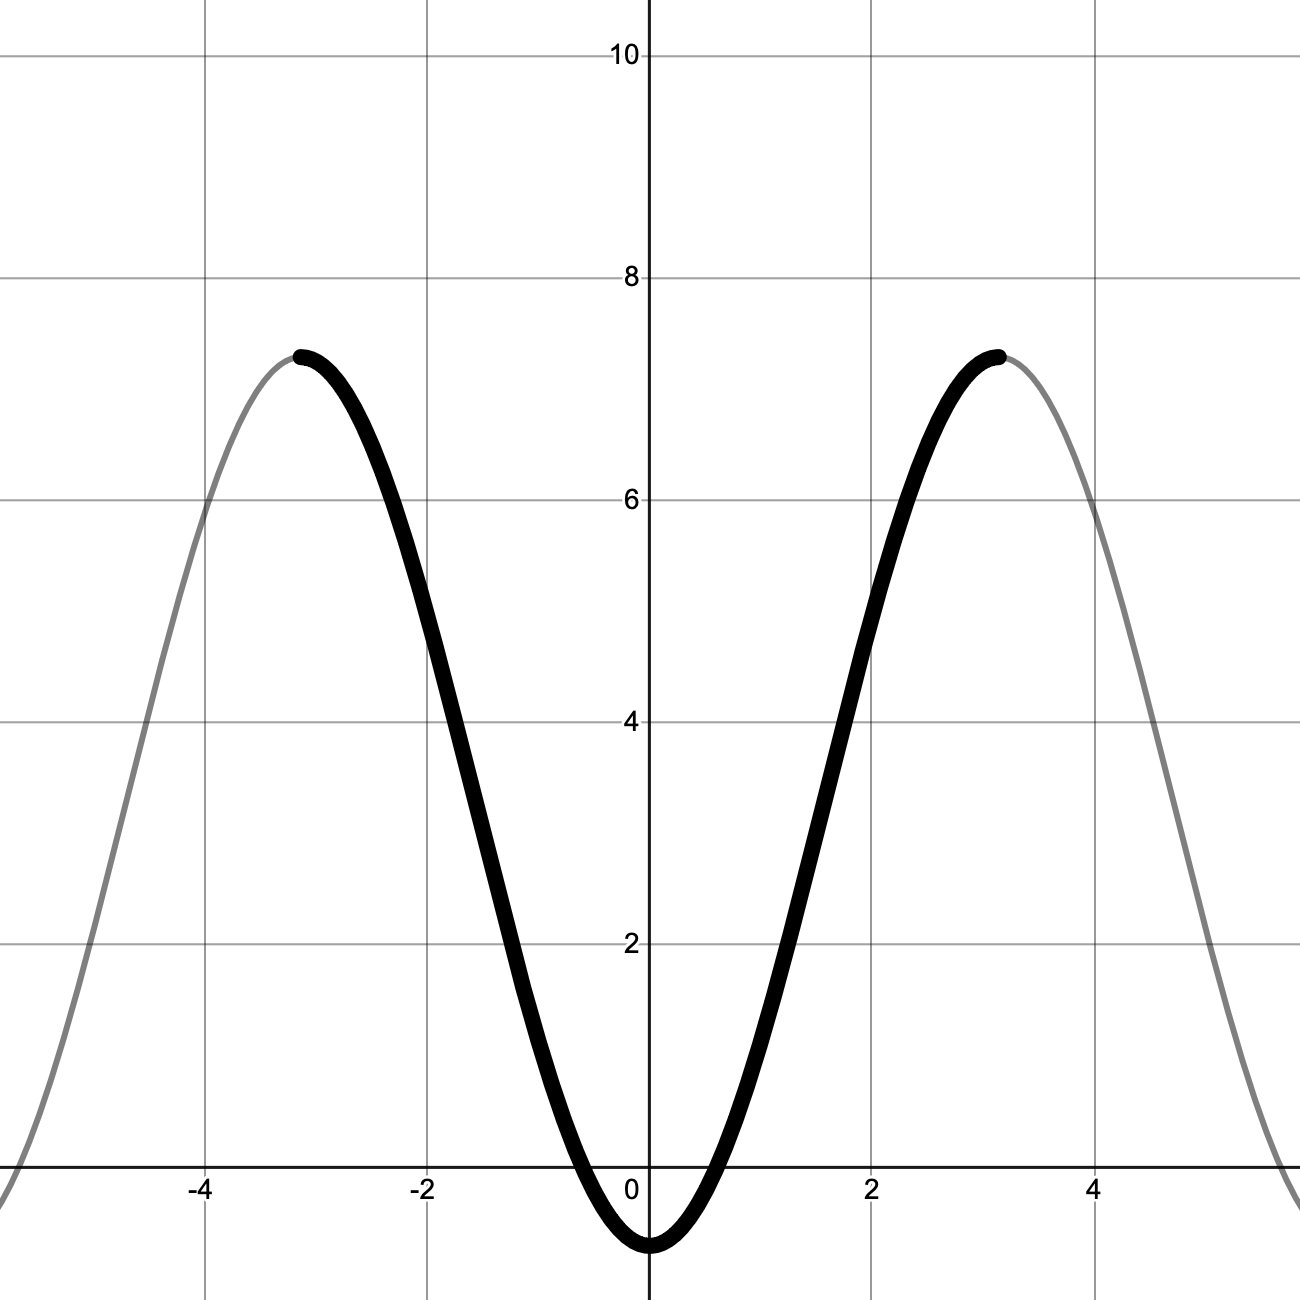
\includegraphics[width=40mm]{Images/simple_1.png} &
  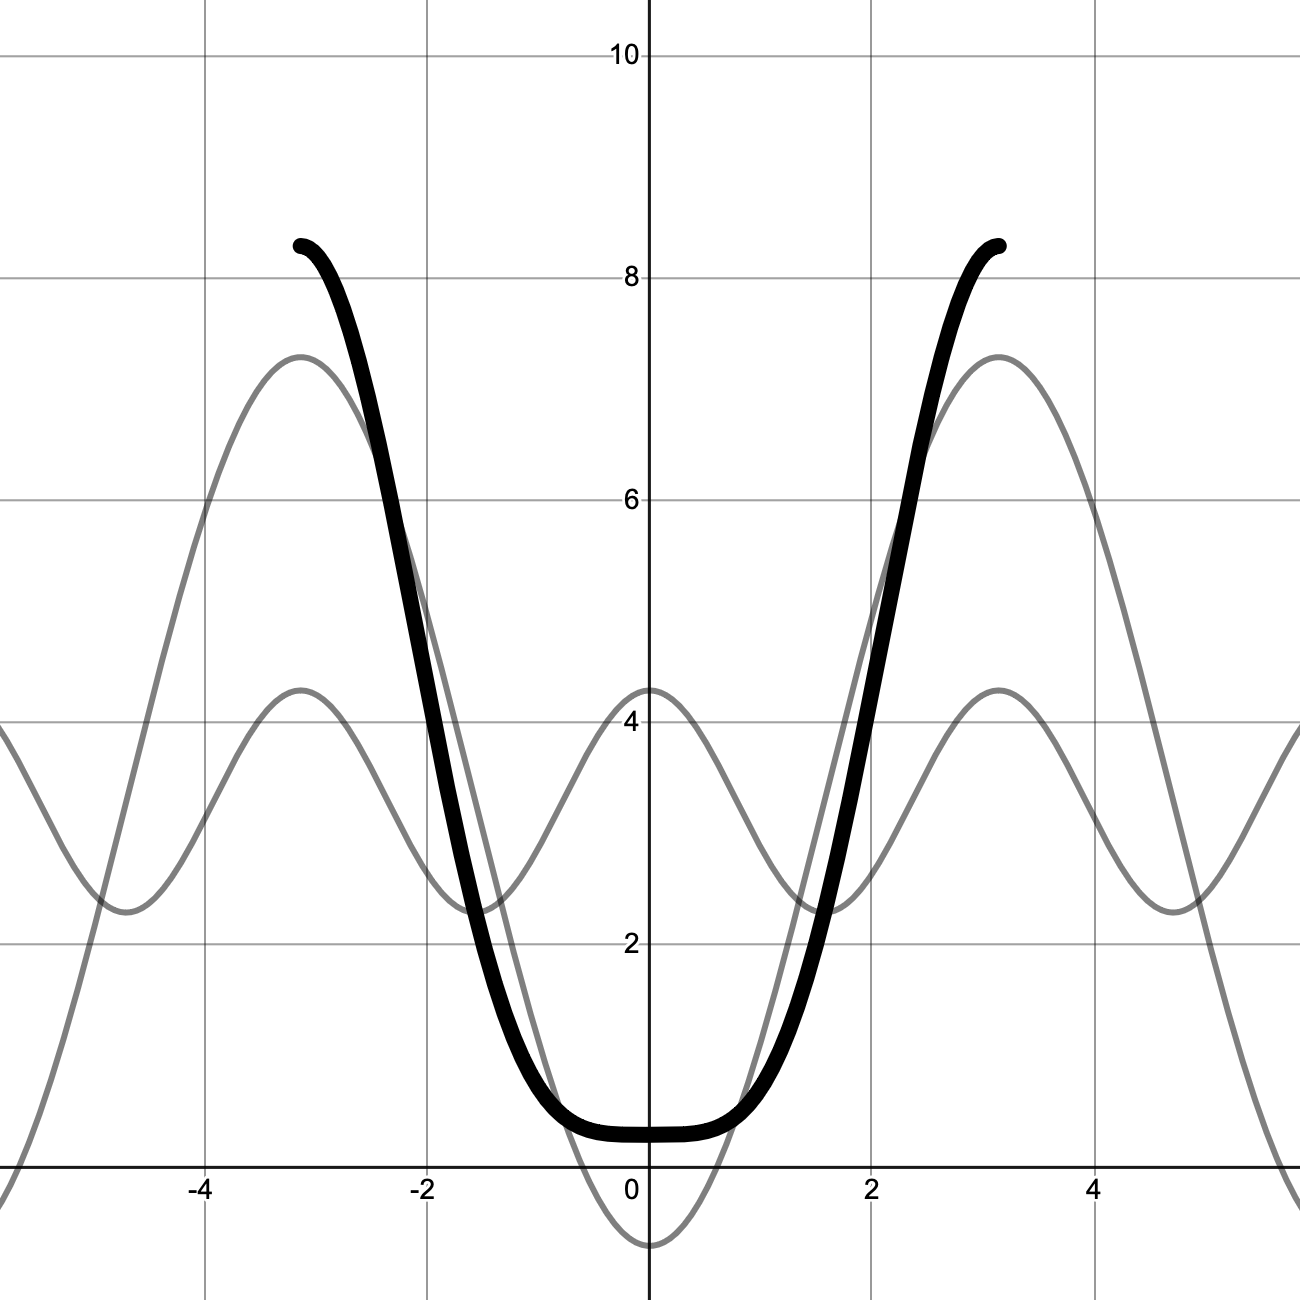
\includegraphics[width=40mm]{Images/simple_2.png} &
  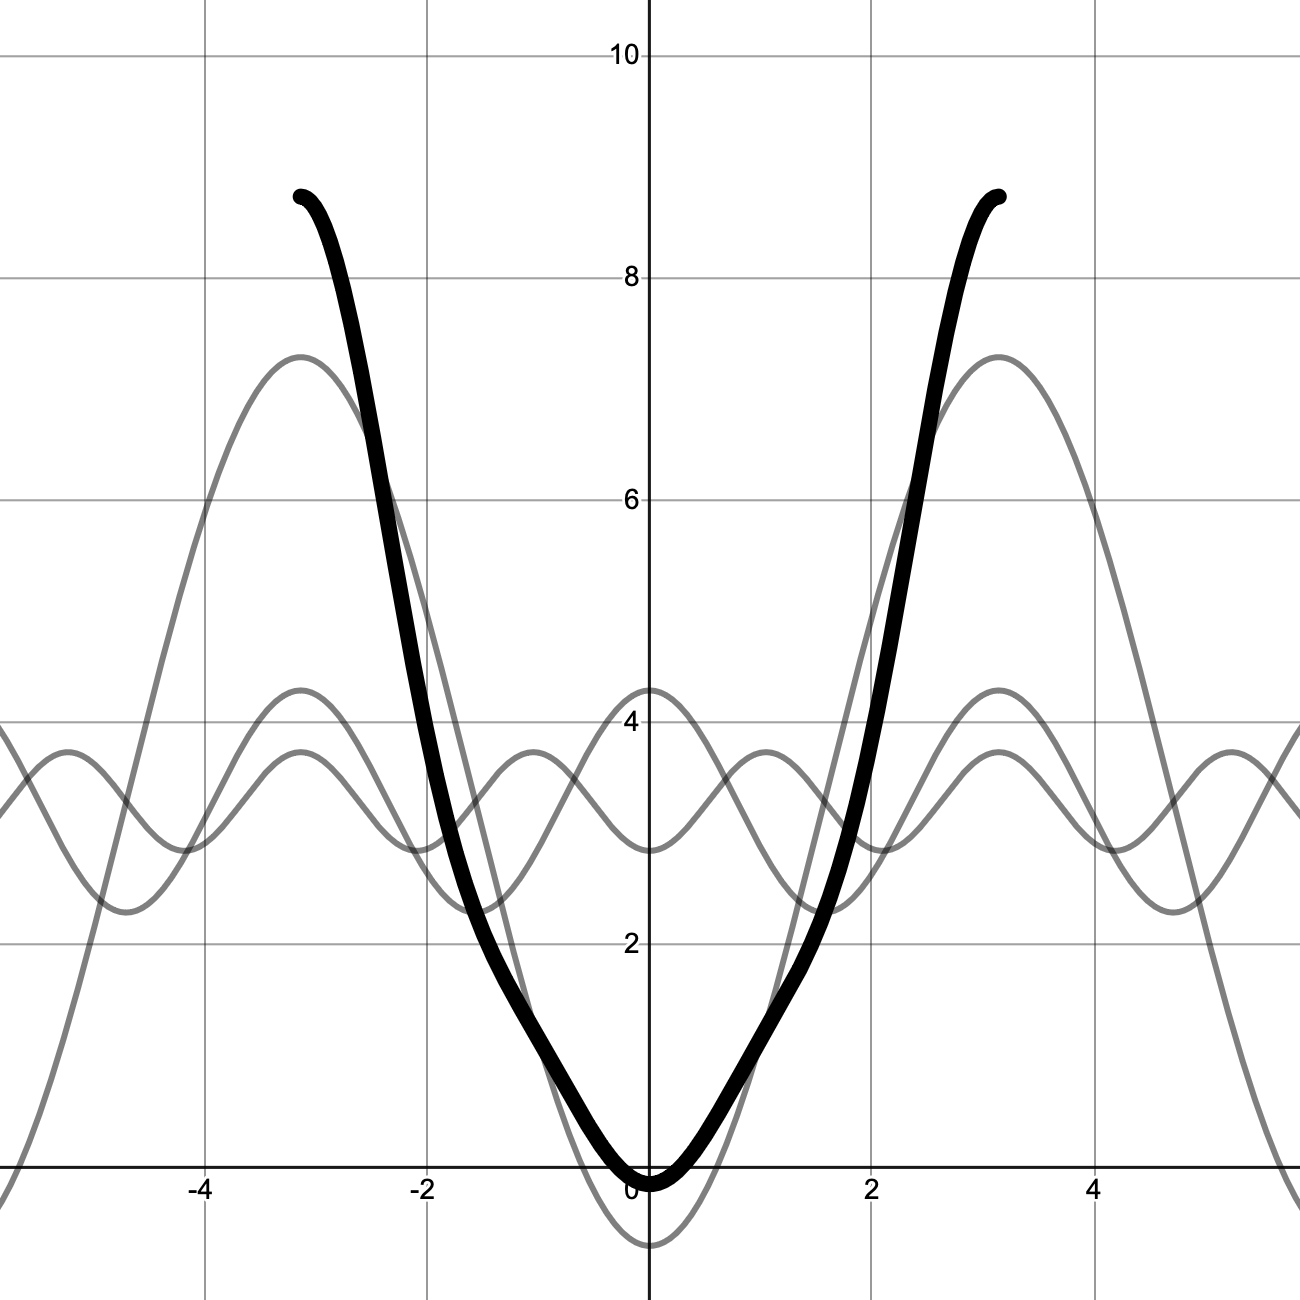
\includegraphics[width=40mm]{Images/simple_3.png} \\
  $n=1$ & $n=2$ & $n=3$\\[6pt]
%   \end{tabular}
% \end{figure}
% \newpage 
%   \begin{figure}[h!]
% \centering
% \begin{tabular}{ccc}
  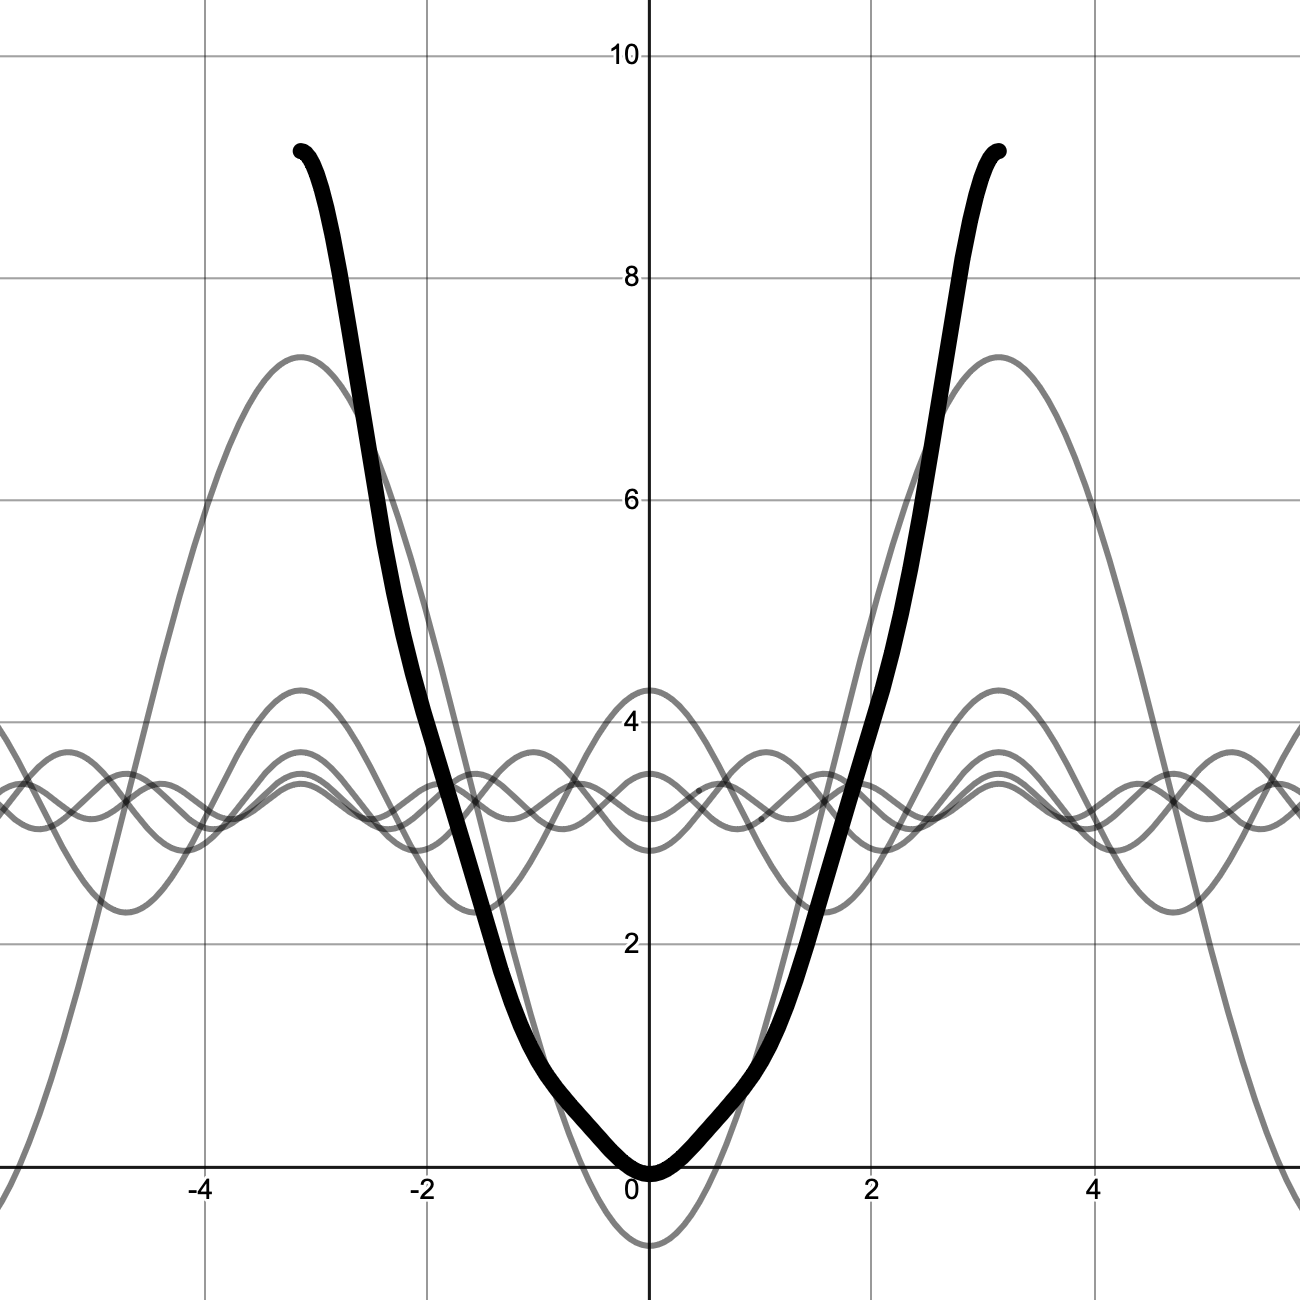
\includegraphics[width=40mm]{Images/simple_5.png} &
  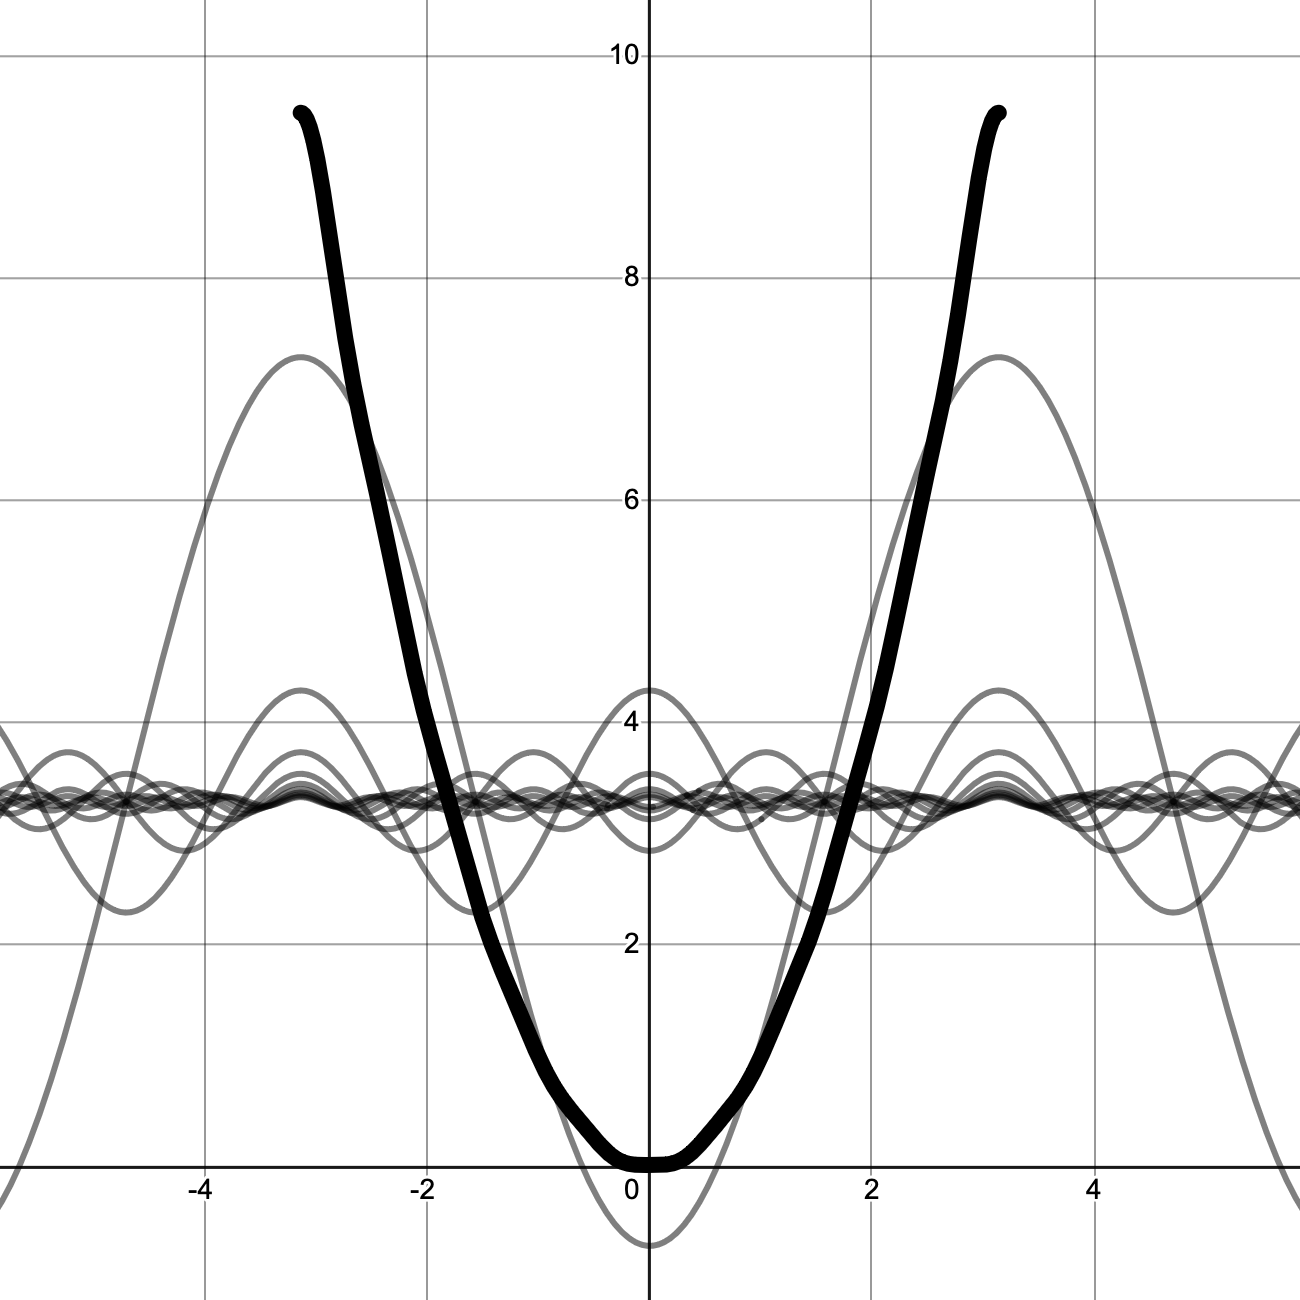
\includegraphics[width=40mm]{Images/simple_10.png} &
  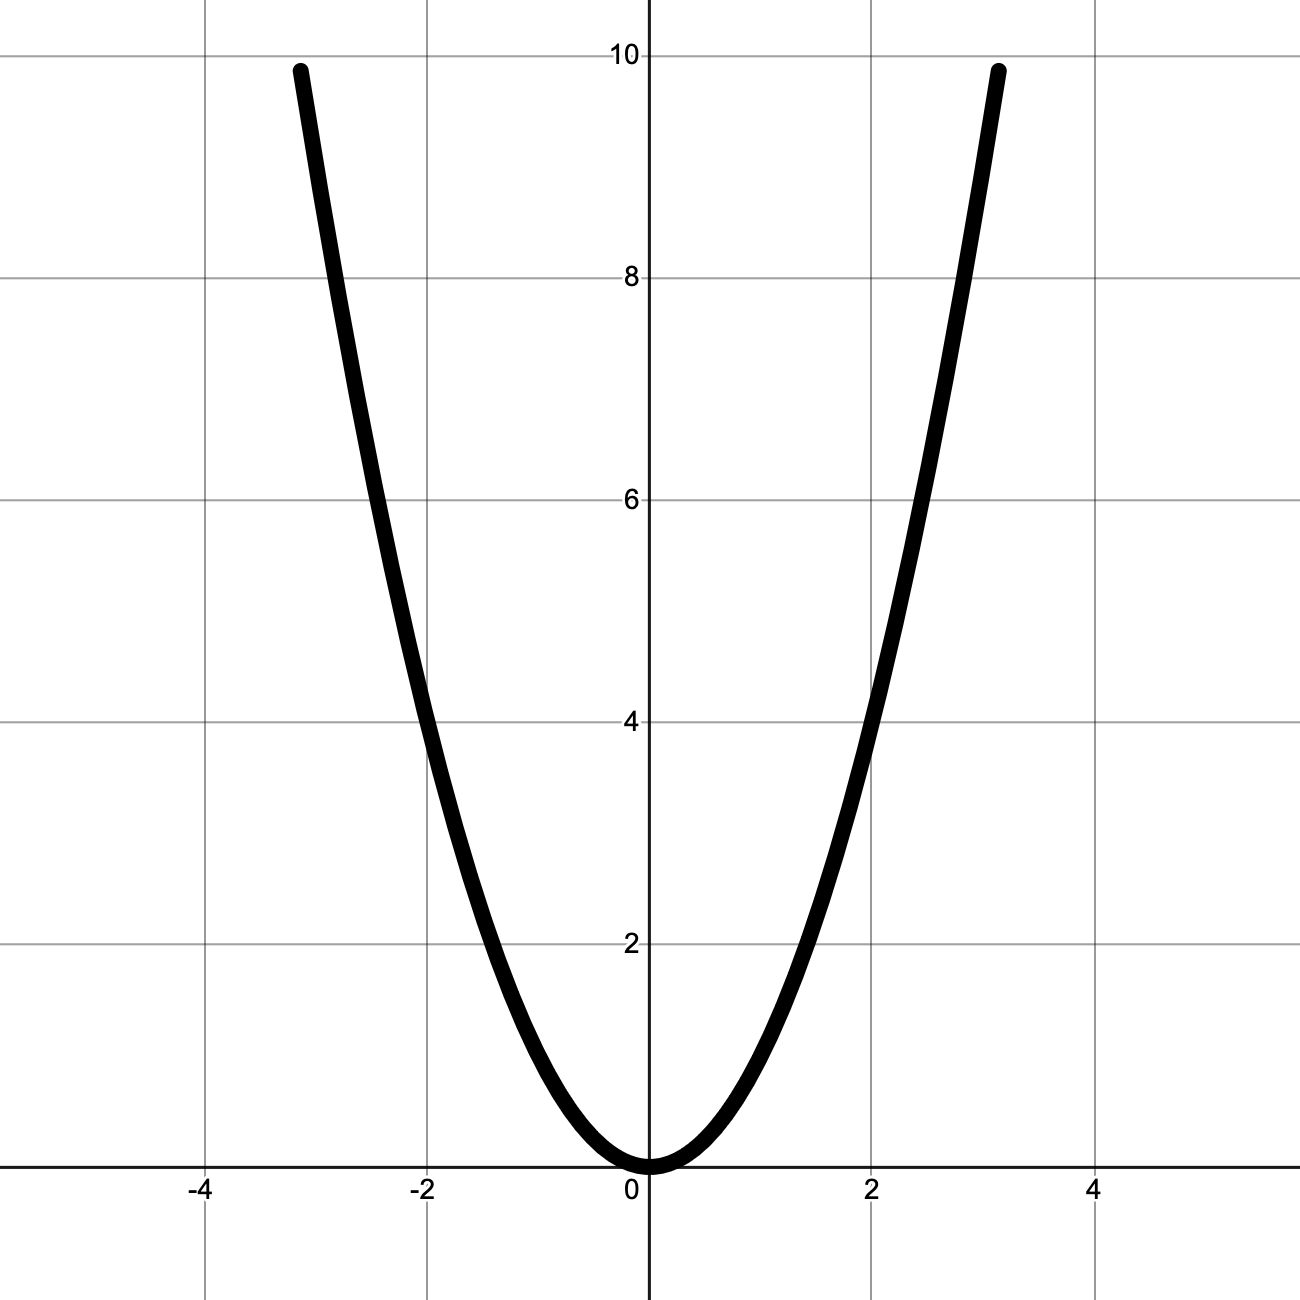
\includegraphics[width=40mm]{Images/simple_full.png} \\
  $n=5$ & $n=10$ & $n\to\infty$\\[6pt]
\end{tabular}
\caption{\centering The Fourier Series representation of the function $f(x)=x^2$.}
\label{fig:simple}
\end{figure}

In Figure \ref{fig:simple}, we see the Fourier Seires representation of $f$ where the thicker line represents the value of the summation for different values of $n$ while the more faint lines are the individual terms in each summation. We have shown how an everywhere-continuous and differentiable function such as $f(x)=x^2$ can be represented by a Fourier series. This idea extends to any function $f$ that behaves in a similar way. Further, Section \ref{sawtooth} shows that the Fourier Transform is useful for discontinuous or non-differentiable functions.

\subsection{Generalizing the Interval}\label{bounds}
    As we have seen in previous sections, the Fourier Transform is an ingenious technique to represent any given function as an infinite trigonometric series. In Section \ref{deriving}, we showed the derivation of the Fourier Series representation, assuming that the given function $f$ was defined over the interval $[-\pi,\pi]$. Section \ref{x2} outlines how an inherently non-periodic function like $f(x) = x^2$ can be made periodic and represented by a Fourier Series. Though remarkable, restricting the function $f$ to this interval limits the utility of the Transformation. Naturally, the question arises whether it is possible to create a Fourier Series representation over any arbitrary interval in $\R$. Unsurprisingly, the answer is yes.  

    \begin{lemma}\label{lem:bounds}
        Let $f:[a,b]\to\R$ be an arbitrary function. If $f$ can be expressed as an infinite trigonometric series in the form 
        \begin{equation}
            \label{eqn:fourier2}
            f(x) = a_0 + \sum_{n=1}^\infty a_n\cos\left(\dfrac{2\pi nx}{b-a}\right) + b_n\sin\left(\dfrac{2\pi nx}{b-a}\right),
            \end{equation}
        then the coefficients  $a_0$, $a_n$, and $b_n$ are given by
        \begin{enumerate}[(i)]
            \item $a_0=\frac{1}{b-a}\int_{a}^{b}f(x)dx$,
            \item $a_n=\int_{a}^{b}f(x)\cos\left(\frac{2\pi nx}{b-a}\right)dx$,
            \item $b_n=\int_{a}^{b}f(x)\sin\left(\frac{2\pi nx}{b-a}\right)dx.$
        \end{enumerate}
    \end{lemma}
This Lemma follows as a results of Theorem \ref{deriving}.
\subsection{Fourier Series of a Piecewise Function}\label{sawtooth}
In a previous section, we showed the derivation of the Fourier Series representation for $f(x)=x^2$, an everywhere continuous and differentiable function. To show the true capability of the Fourier Transform, consider the function $g:[-1,1]\to\R$ defined by

\begin{minipage}{0.5\textwidth}
    $$g(x) = \begin{cases}
        0, & -1 \leq x < 0 \\
        x, & 0 \leq x < 1.
    \end{cases}$$
\end{minipage}
\begin{minipage}{0.5\textwidth}
        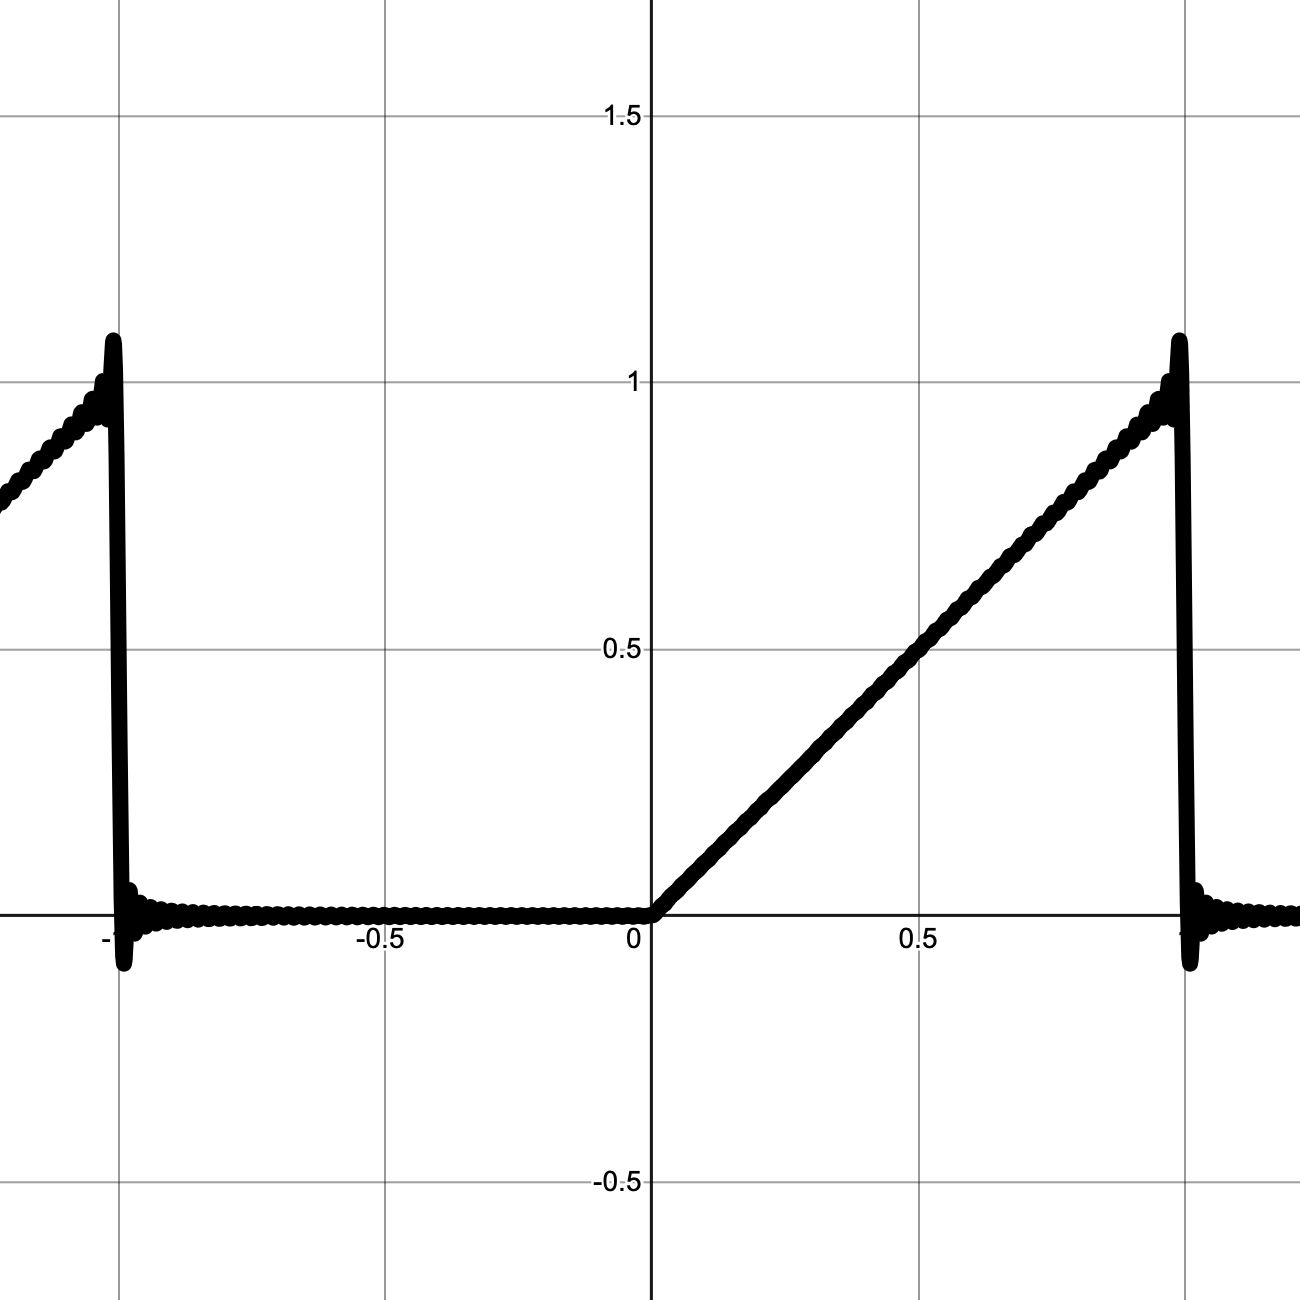
\includegraphics[width=35mm]{Images/complex_full.png}
\end{minipage}
Note that we have defined $g$ over the interval $[-1,1]$ but have represented it as a periodic function. By nature of the Fourier Transform, the resulting function's representation is periodic. This is simply something to consider when building the series. Using the generalized Fourier Series representation shown in Lemma \ref{lem:bounds}, let $a=-1$ and $b=1$. It follows that $$a_0=\dfrac{1}{b-a}\int_{a}^{b}g(x)dx = \dfrac{1}{2}\int_{-1}^{1}g(x)dx= \dfrac{1}{2}\left[\int_{-1}^{0}0\ dx + \int_{0}^{1}x\ dx\right]= \dfrac{1}{2}\left[\dfrac{1}{2}x^2\right]_{0}^{1} = \dfrac{1}{4}.$$
To derive $a_n$, we have that
\begin{align*}
    a_n &= \int_{a}^{b}g(x)\cos\left(\dfrac{2\pi nx}{b-a}\right)dx\\
        &= \int_{-1}^{1}g(x)\cos\left(\pi nx\right)dx\\
        &= \int_{-1}^{0}0\cdot\cos\left(\pi nx\right)dx + \int_{0}^{1}x\cos\left(\pi nx\right)dx\quad (\dagger)\\
        &= \left[\dfrac{x}{\pi n}\sin(\pi nx) + \dfrac{1}{\pi^2 n^2}\cos(\pi nx)\right]_0^1\\
        &= \left[\dfrac{1}{\pi n}\sin(\pi n) + \dfrac{1}{\pi^2 n^2}\cos(\pi n)\right] - \left[0 + \dfrac{1}{\pi^2 n^2}\cos(0)\right]\\
        &= \dfrac{1}{\pi n}\sin(\pi n) + \dfrac{1}{\pi^2 n^2}\cos(\pi n) -\dfrac{1}{\pi^2 n^2}\\
        &= \dfrac{(-1)^n-1}{\pi^2 n^2}.
\end{align*}
where $(\dagger)$ was computed using integration by parts. 

Similarly, to derive $b_n$, we have that 
\begin{align*}
    b_n &= \int_{a}^{b}g(x)\sin\left(\dfrac{2\pi nx}{b-a}\right)dx\\
        &= \int_{-1}^{1}g(x)\sin\left(\pi nx\right)dx\\
        &= \int_{-1}^{0}0\cdot\sin\left(\pi nx\right)dx + \int_{0}^{1}x\sin\left(\pi nx\right)dx\quad (\dagger)\\
        &= \left[-\dfrac{x}{\pi n}\cos(\pi nx) + \dfrac{1}{\pi^2 n^2}\sin(\pi nx)\right]_0^1\\
        &= \left[-\dfrac{1}{\pi n}\cos(\pi n) + \dfrac{1}{\pi^2 n^2}\sin(\pi n)\right] - \left[0 + \dfrac{1}{\pi^2 n^2}\sin(0)\right]\\
        &= -\dfrac{1}{\pi n}\cos(\pi n)\\
        &= -\dfrac{(-1)^n}{\pi n},
\end{align*}

again where $(\dagger)$ was computed using integration by parts. From the work above, we have that our original function $g$ can be represented by the Fourier Series $$g(x) =\dfrac{1}{4} + \sum_{n=1}^\infty \dfrac{(-1)^n-1}{\pi^2 n^2}\cos(\pi nx) - \dfrac{(-1)^n}{\pi n}\sin(\pi nx)$$
In the following images, we can visualize the Fourier Series along different values of $n$. As $n\to\infty$, we observe how the representation approaches the original function $g$. 
\begin{figure}[ht!]
\centering
\begin{tabular}{ccc}
  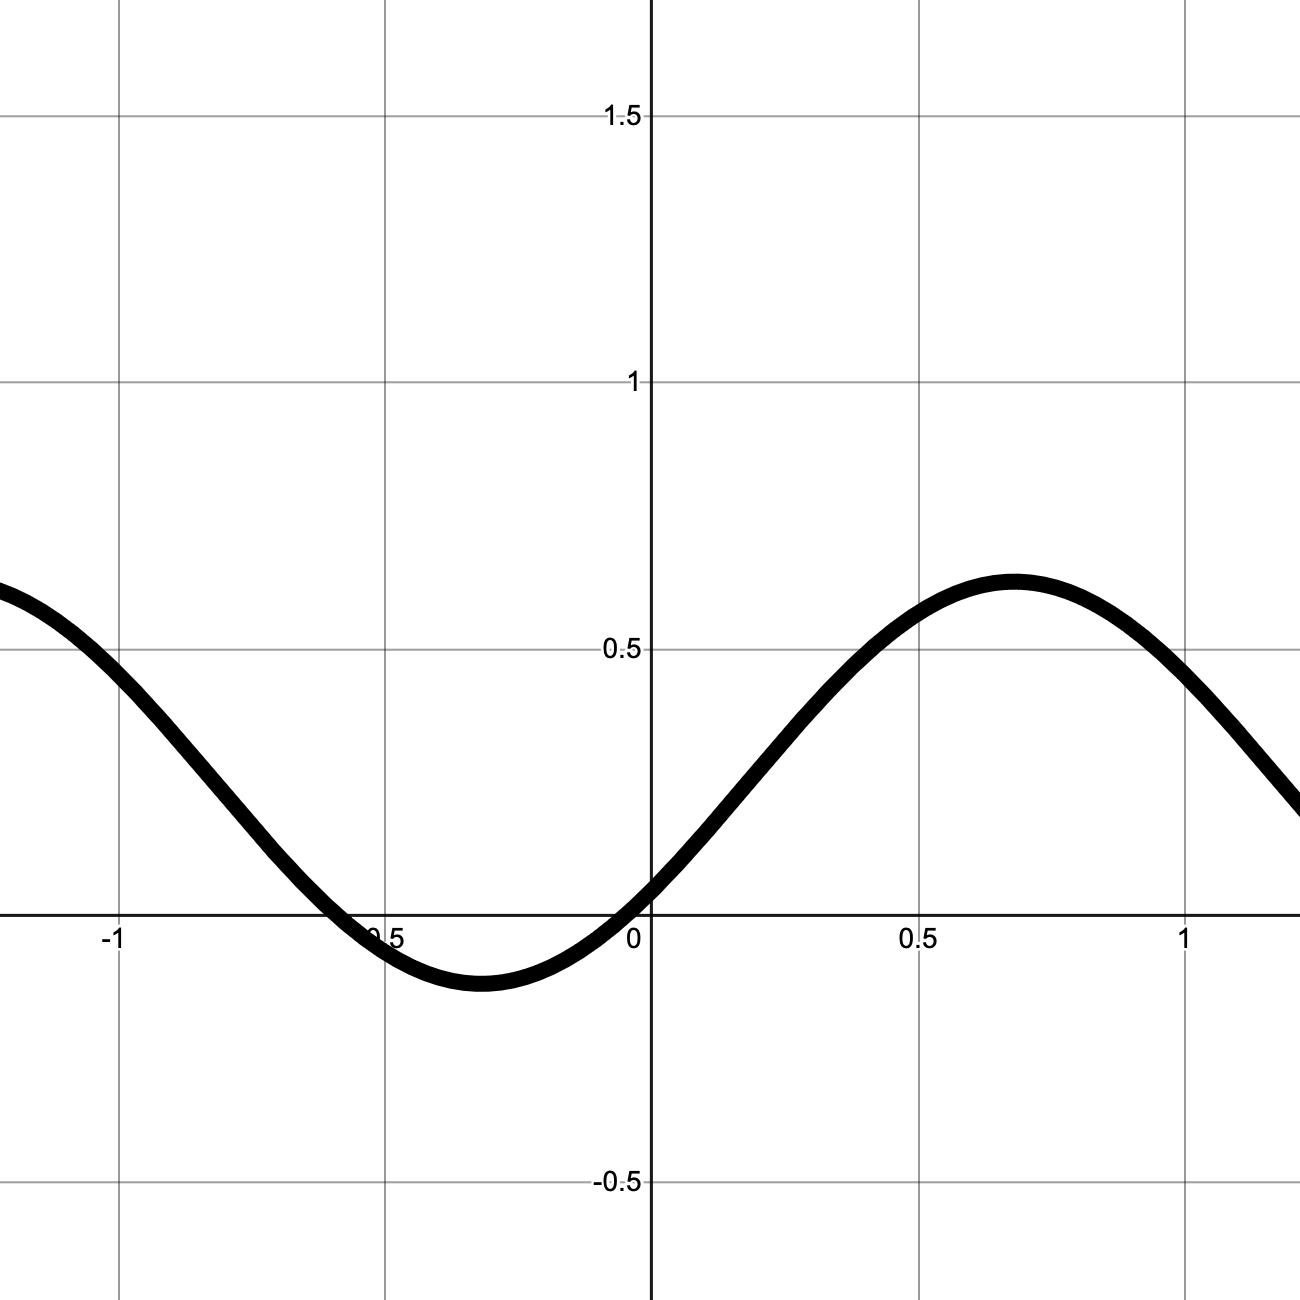
\includegraphics[width=40mm]{Images/complex_1.png} &
  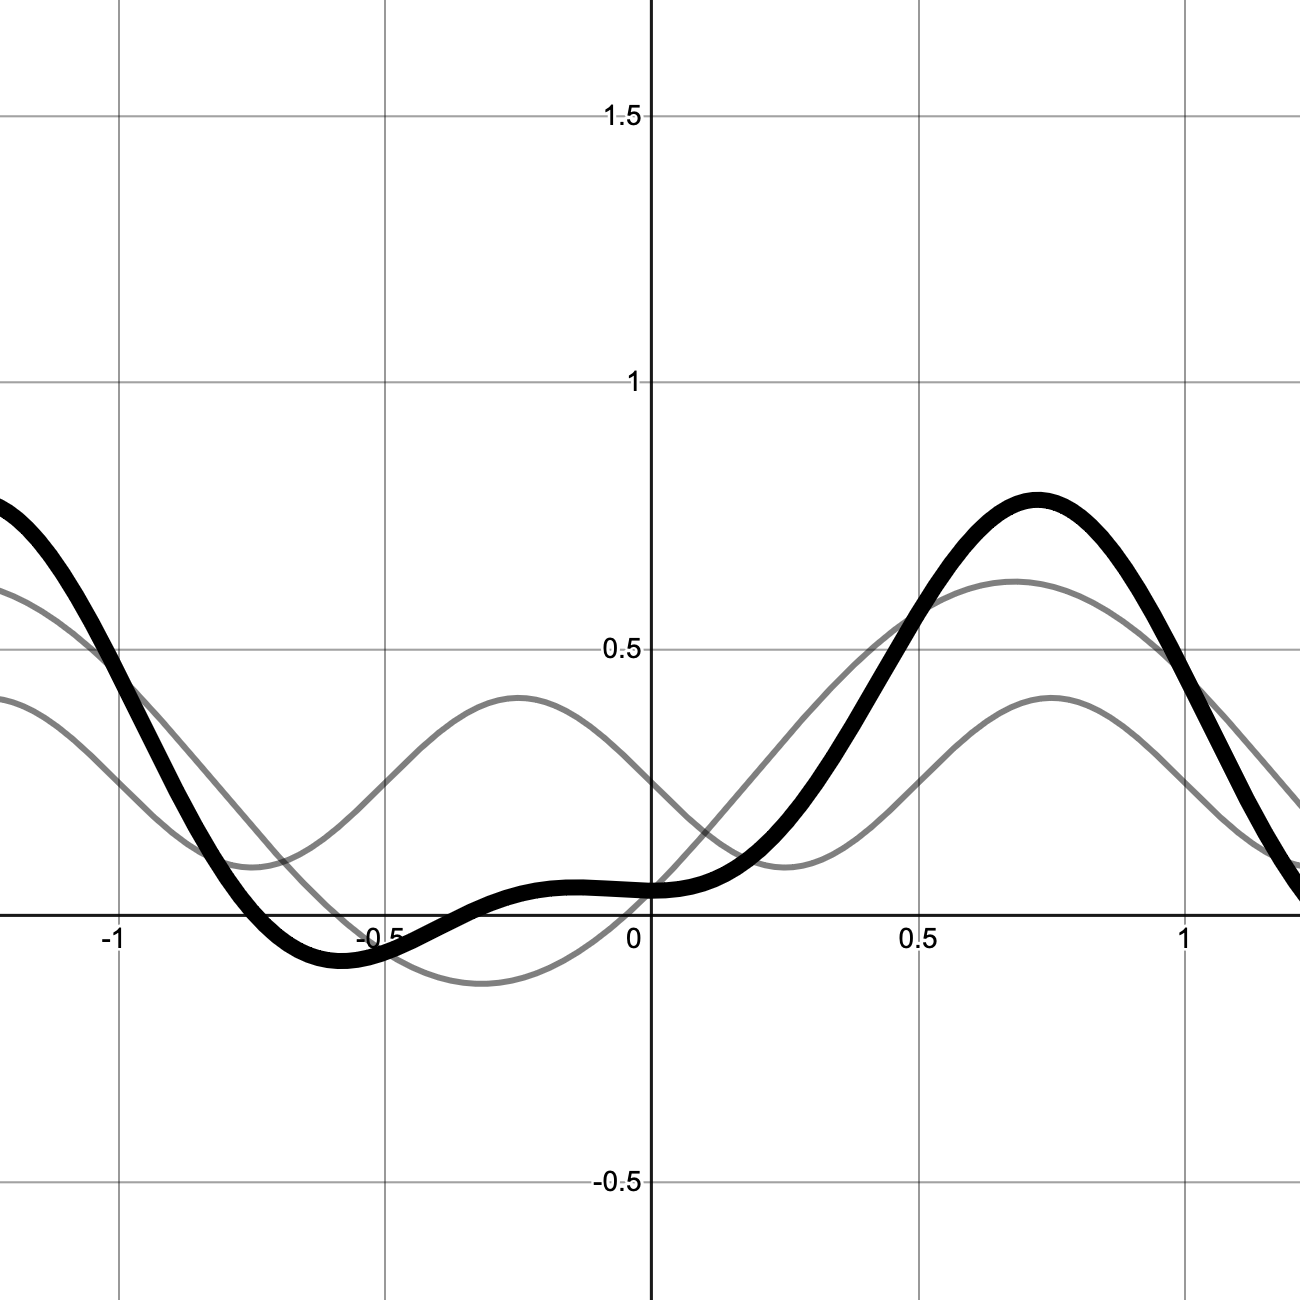
\includegraphics[width=40mm]{Images/complex_2.png} &
  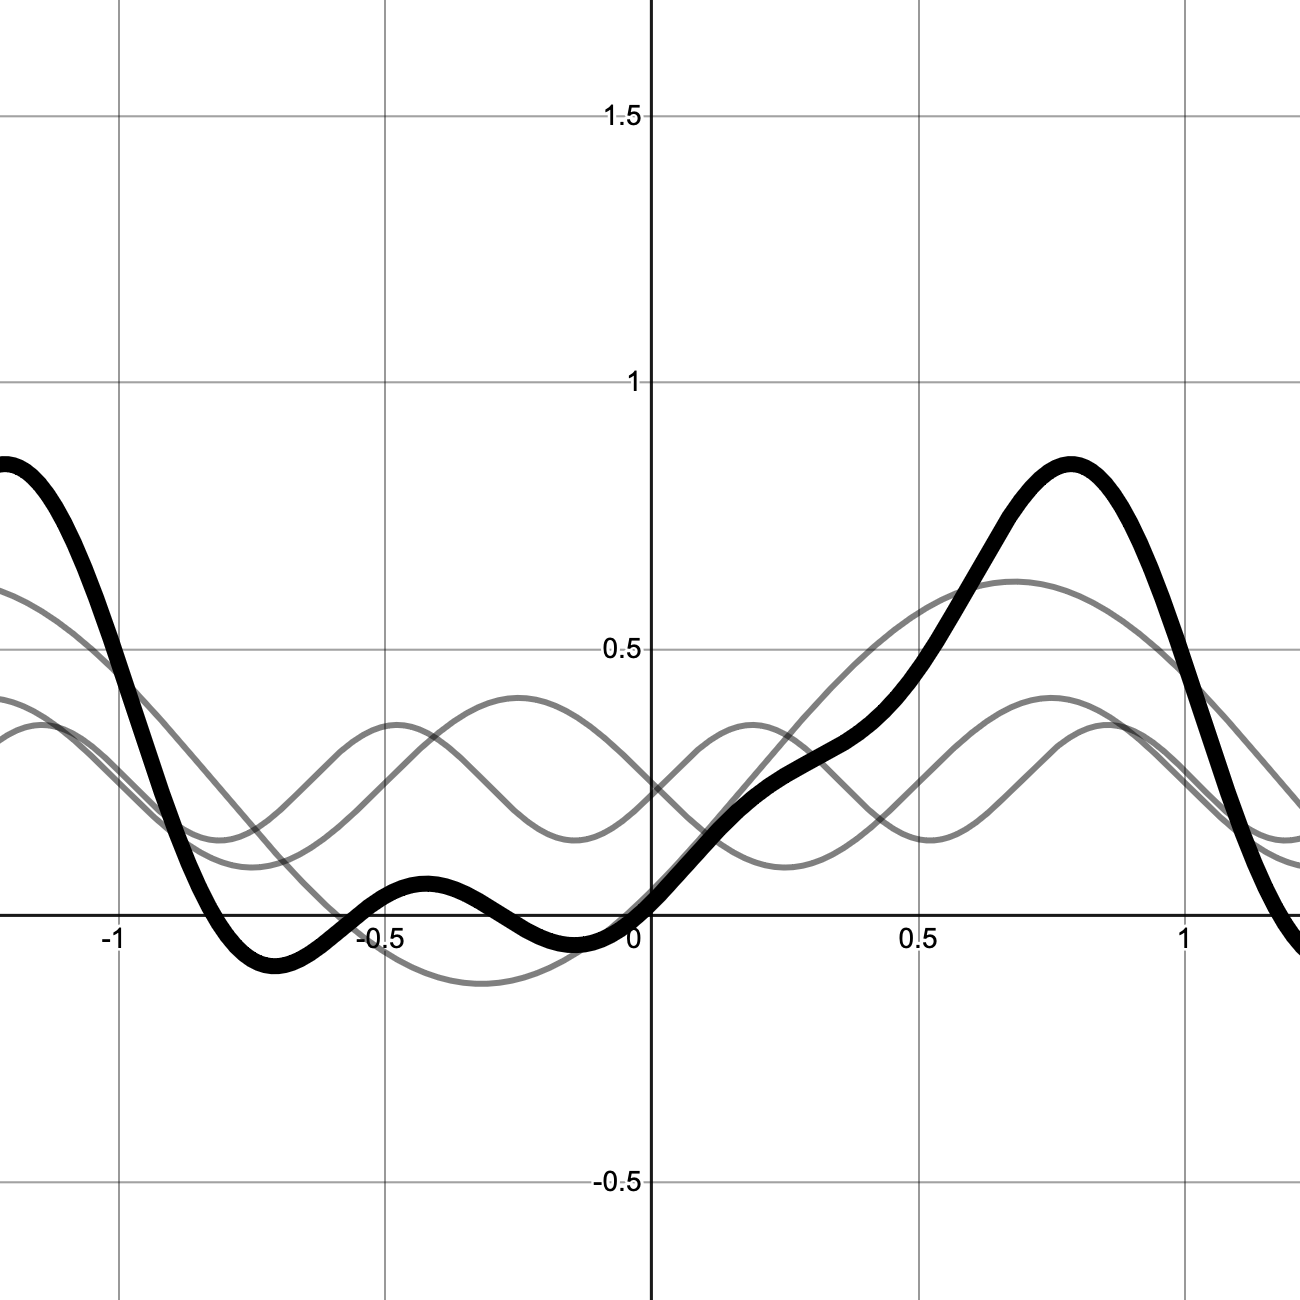
\includegraphics[width=40mm]{Images/complex_3.png} \\
  $n=1$ & $n=2$ & $n=3$\\[6pt]
% \end{tabular}
% \end{figure}
% % \newpage
%   \begin{figure}[h!]
% \centering
% \begin{tabular}{ccc}
  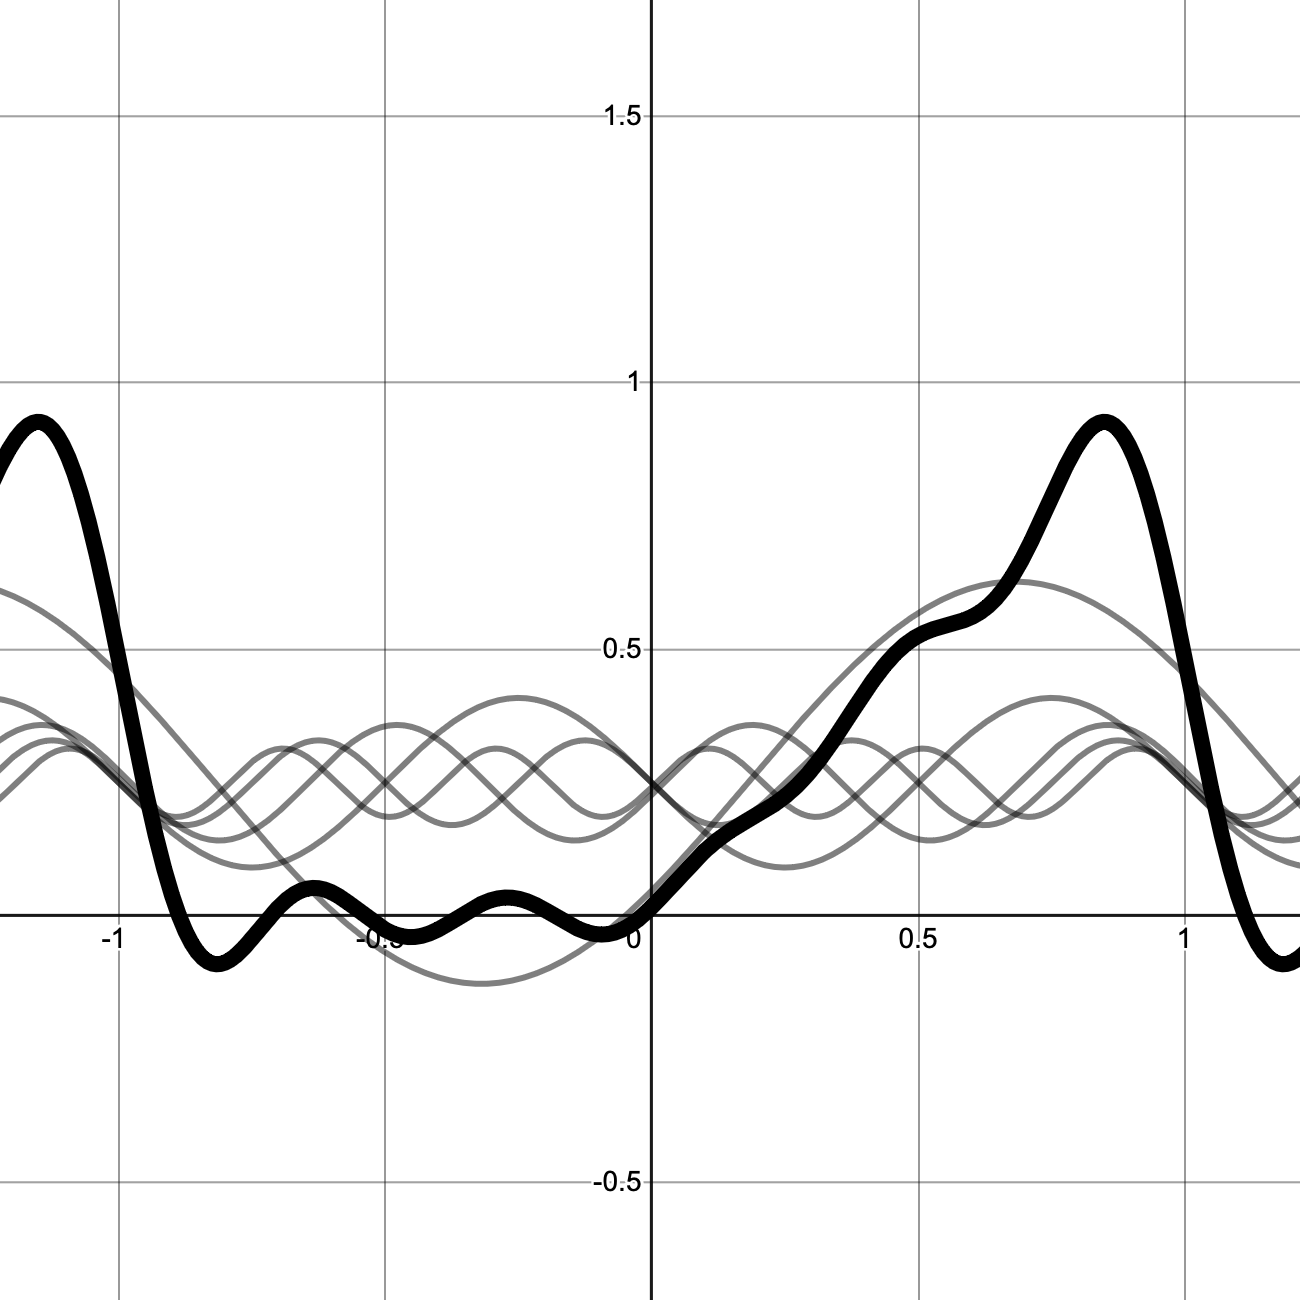
\includegraphics[width=40mm]{Images/complex_5.png} &
  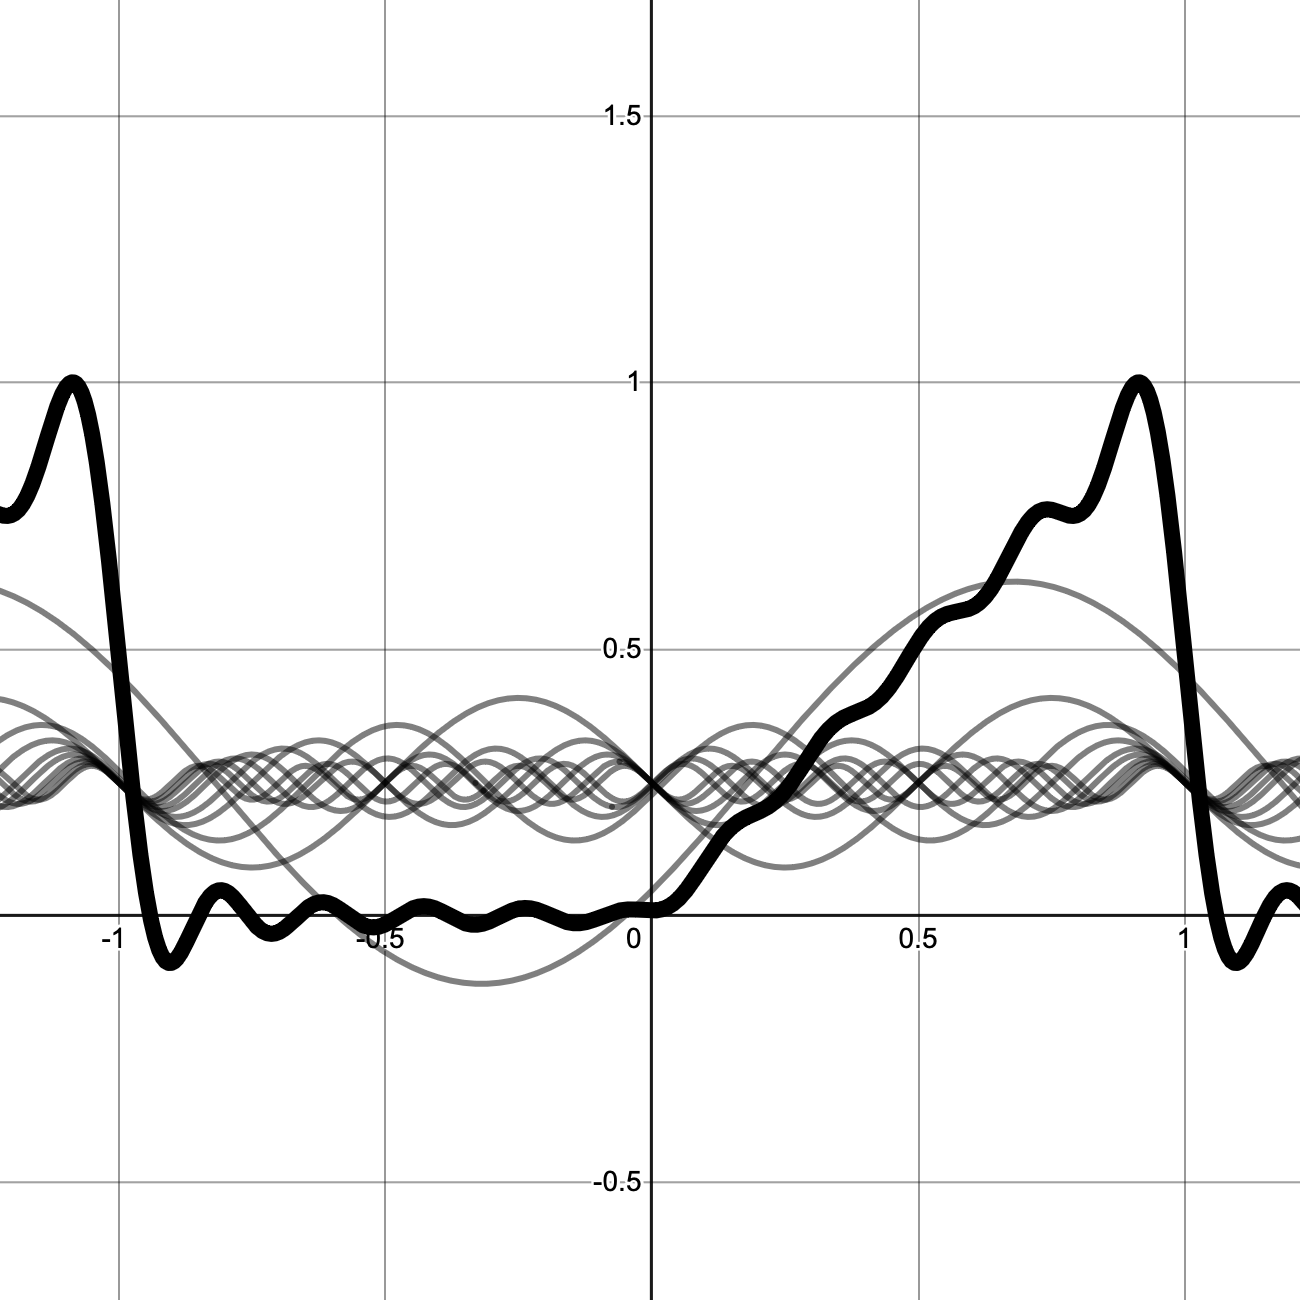
\includegraphics[width=40mm]{Images/complex_10.png} &
  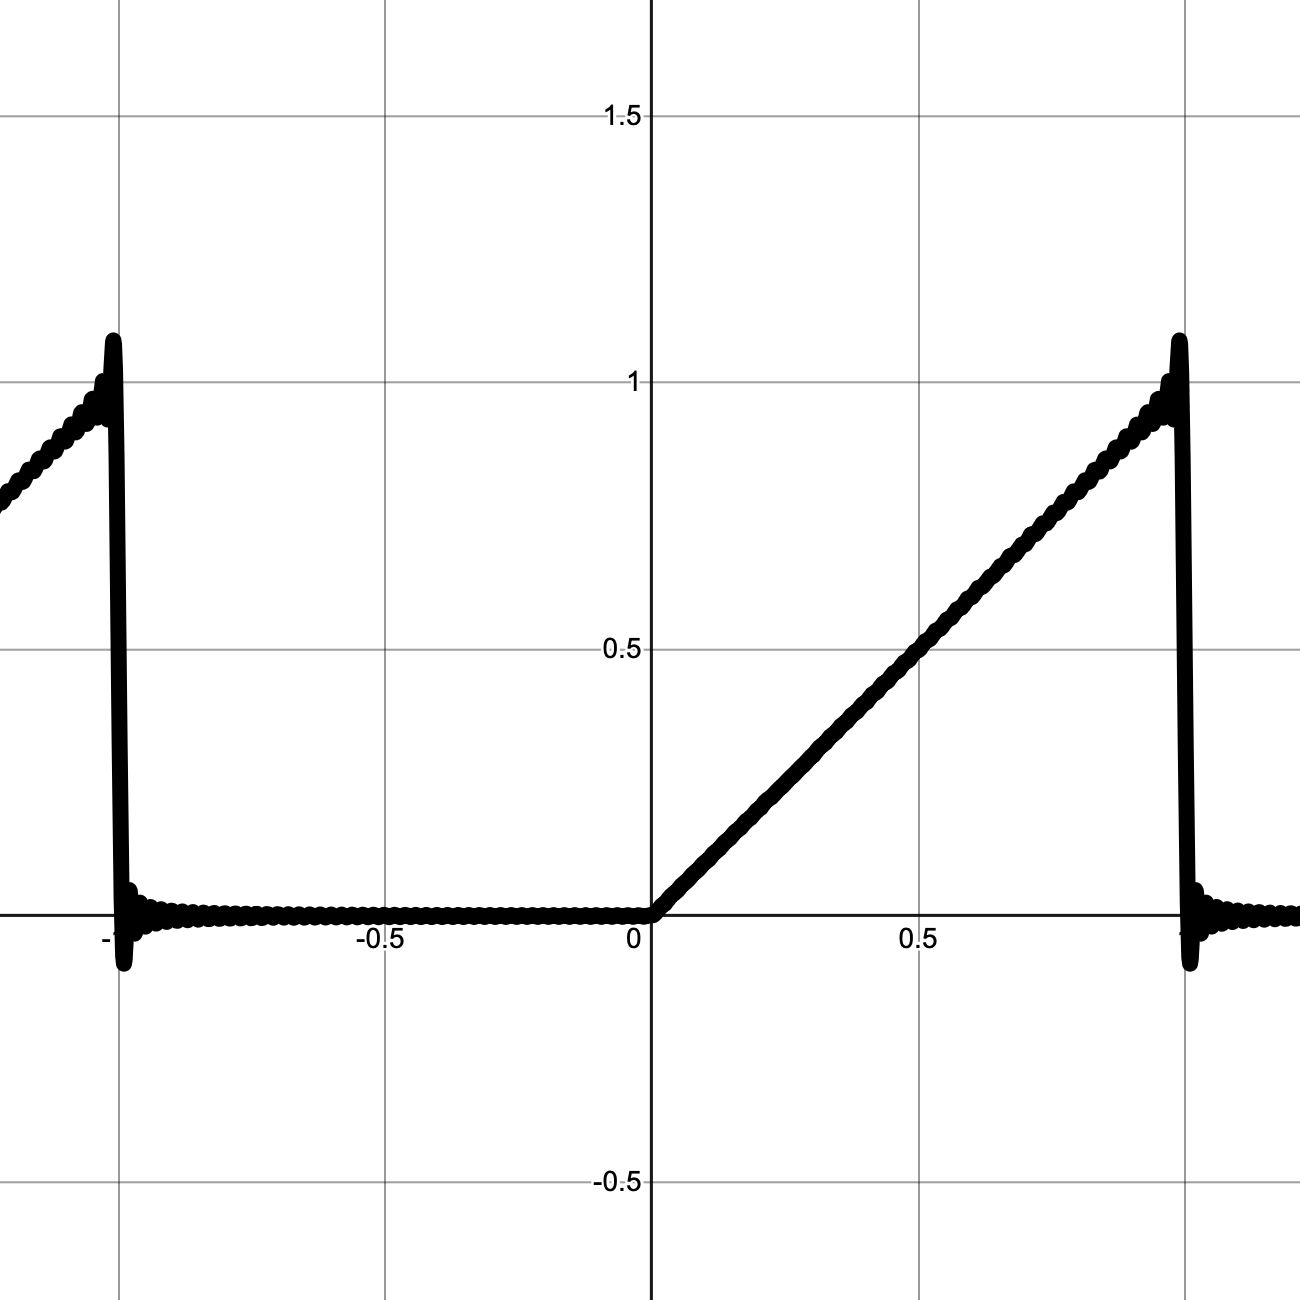
\includegraphics[width=40mm]{Images/complex_full.png} \\
  $n=5$ & $n=10$ & $n\to\infty$\\[6pt]
\end{tabular}
\caption{\centering The Fourier Series Representation of the Sawtooth function $g$.}
\label{fig:complex}
\end{figure}

In Figure \ref{fig:complex}, we see the approximation of the function $g$ where the thicker line represents the value of the summation for different values of $n$ while the more faint lines are the individual terms in each summation. Importantly, Figure \ref{fig:complex} highlights the superposition of unique sinusoidal waves. Each sequential term in the summation either adds to or reduces the height of prior terms.

\section{Continuity and Differentiability}

\subsection{Continuity of a Fourier Series}
As mentioned in the introduction, one of the defining characteristics of the Fourier Transform is the property of continuity. In this section, we demonstrate how a continuous, differentiable function like $f(x)=x^2$ can be represented by the continuous series derived in Section \ref{x2}. To prove this property, first consider the following theorems which we will use to prove the continuity of the Fourier series. 

\begin{theorem}[\textbf{Term-by-term Continuity Theorem} \cite{Abbott}]\label{thm:continuity}
    Let $f_n$ be continuous functions defined on a set $A\subseteq\R$, and assume $\sum_{n=1}^\infty f_n$ converges uniformly on $A$ to a function $f$. Then, $f$ is continuous on $A$.
\end{theorem}

\begin{corollary}[\textbf{Weierstrass M-Test} \cite{Abbott}]\label{weier}
    For each $n\in \N$, let $f_n$ be a function defined on a set $A\subseteq \R$, and let $M_n>0$ be a real number satisfying \[|f_n(x)|\leq M_n\] for all $x\in A$. If $\sum_{n=1}^\infty M_n$ converges, then $\sum_{n=1}^\infty f_n$ converges uniformly on $A$.
\end{corollary}
 
\begin{eg}
    Show that the Fourier series representation of $f(x)=x^2$ is continuous on the interval $[-\pi,\pi]$. 
\end{eg}
\begin{proof}
    Recall the Fourier series representation of $f(x)=x^2$ from Section 4.1, \[f(x)=\dfrac{\pi^2}{3}+\sum_{n=1}^\infty \dfrac{4(-1)^n}{n^2}\cos(nx).\] Notice that $f=a_0+\sum_{n=1}^\infty f_n$ where $f_n$ is defined as \[f_n= \dfrac{4(-1)^n}{n^2}\cos(nx).\] By the Algebraic Differentiability Theorem \cite{Abbott}, $f$ is differentiable if both $a_0$ and $\sum_{n=1}^\infty f_n$ are differentiable. Therefore, the leading constant $a_0$ is negligible.
    
    To determine if the series is continuous using Theorem \ref{thm:continuity}, we must first need to prove that each $f_n$ is continuous on the interval $[-\pi,\pi]$. From calculus, we know that $\cos(nx)$ is continuous for all $x\in [-\pi,\pi]$, and for all $n\in\N$, $\frac{4(-1)^n}{n^2}$ evaluates to a real number. Thus $f_n$ is continuous on $[-\pi,\pi]$. 
    
    Now, we need to prove that $\sum_{n=1}^\infty f_n$ converges uniformly on the interval $[-\pi,\pi]$ using Corollary \ref{weier}. Let $M_n= 4/n^2$ and observe that $(M_n)\to 0$. Then for all $x\in [-\pi,\pi]$,
    \begin{align*}
        |f_n(x)| &= \left|\frac{4(-1)^n\cos(nx)}{n^2}\right| \\
        &\leq \left|\frac{4(-1)^n}{n^2}\right|\\
        &= \frac{4}{n^2}\\
        &= M_n.
    \end{align*}
    Thus, $|f_n(x)|\leq M_n$ for all $x\in [-\pi,\pi]$. Therefore $\sum_{n=1}^\infty f_n$ converges uniformly on the interval by Corollary \ref{weier}. Finally, we have both conditions met for Theorem \ref{thm:continuity}, and conclude that $f$ is continuous on the interval $[-\pi,\pi]$. 
\end{proof}

\subsection{Differentiability of a Piecewise Function}
 Before the mathematical revolution of the late 18th century, most of calculus was concerned only with polynomial and trigonometric functions. Inherently, these functions are everywhere continuous and infinitely differentiable, making those properties trivial. However, as the definition of the function was reshaped by mathematicians like Dirichlet, differentiability became increasingly relevant \cite{Abbott}. In this section, we demonstrate how a discontinuous, non-differentiable function like $g$ in Section \ref{sawtooth} can be made both continuous and infinitely differentiable by the Fourier Transform. To prove this property, first consider the following theorem. 
\begin{theorem}[\textbf{Term-by-term Differentiablility Theorem}] \cite{Abbott}\label{thm:diff}
    Let $f_n$ be differentiable functions defined on an interval $A$, and assume $\sum_{n=1}^\infty f'_n(x)$ converges uniformly to a limit $g(x)$ on $A$. If there exists a point $x_0\in [a,b]$ where $\sum_{n=1}^\infty f_n(x_0)$ converges, then the series $\sum_{n=1}^\infty f_n(x)$ converges uniformly to a differentiable function $f(x)$ satisfying $f'(x)=g(x)$ on $A$.
\end{theorem}

\begin{eg}
    Show that the Fourier Series representation of the Sawtooth Wave from Section \ref{sawtooth} is differentiable on the interval $[-1,1]$.
\end{eg}
\begin{proof}
    Let $g$ be the Fourier Series from Section \ref{sawtooth} where $$g(x) = \dfrac{1}{4} + \sum_{n=1}^\infty \dfrac{(-1)^n-1}{\pi^2 n^2}\cos(\pi nx) - \dfrac{(-1)^n}{\pi n}\sin(\pi nx).$$ Notice that $g = a_0 + \sum_{n=1}^\infty g_n,$ where $g_n$ is defined as $$g_n = \dfrac{(-1)^n-1}{\pi^2 n^2}\cos(\pi nx) - \dfrac{(-1)^n}{\pi n}\sin(\pi nx).$$ By the Algebraic Differentiability Theorem \cite{Abbott}, $g$ is differentiable if both $a_0$ and $\sum_{n=1}^\infty g_n$ are differentiable. Therefore, the leading constant $a_0$ is negligible.

    To apply Theorem \ref{thm:diff}, we must first confirm that the series of derivatives $\sum_{n=1}^\infty g_n'$ converges uniformly on the interval $[-1,1]$. Let $M_n = 1/n$ and observe that $(M_n)\to 0$. Then, for all $x\in[-1,1],$ consider the derivative
    \begin{align*}
        \left|g_n'\right| &= \left|-\dfrac{(-1)^n-1}{\pi n}\sin(\pi nx)-\dfrac{(-1)^n}{\pi n}\cos(\pi nx)\right|\\
            &= \left|\dfrac{1-(-1)^n}{\pi n}-\dfrac{(-1)^n}{\pi n}\right|\\
            &= \left|\dfrac{1}{\pi n}\right| < \dfrac{1}{n} =M_n.
    \end{align*}
    By Corollary \ref{weier}, we conclude that $\sum_{n=1}^\infty g_n'$ converges uniformly on the interval $[-1,1]$.

    In addition to the uniform convergence of the series of derivatives $g_n'$, we must show that for some $x_0\in[-1,1]$, the series $\sum_{n=1}^\infty g_n(x_0)$ converges. So, let $x_0 = 0$. Then, $$g_n(x_0) = \dfrac{(-1)^n-1}{\pi^2n^2} < \dfrac{(-1)^n-1}{n^2}<\dfrac{(-1)^n}{n^2}\leq\dfrac{1}{n^2}.$$ Therefore, $\sum_{n=1}^\infty g_n(x_0)$ converges by the Comparison Test \cite{Abbott}. Finally, we have met the requirements to apply Theorem \ref{thm:diff}. Thus, the function $g$ is differentiable. 
    \end{proof}

In the proof above, we showed that the Fourier Series for $g$ is differentiable. Due to the cyclical nature of trigonometric derivatives, $g$ becomes infinitely differentiable, a remarkable property considering its original piece-wise definition.


\section{Applications}
Now that we have thoroughly demonstrated the foundations, derivations, and utility of the Fourier Transform, we hope to provide some context on a modern day application of Fourier's work. In this section we will briefly discuss the Discrete and Fast Fourier Transforms. This is just one of countless applications that stem from Fourier's work. We cannot understate the usefulness and importance of these applications in technology and modern mathematics. 

\subsection{The Discrete and Fast Fourier Transform}
The Discrete and Fast Fourier Transforms are both techniques utilized often in modern technology. Specifically, these two algorithms aid in audio and image compression for internet communications. As this is a complex, multifaceted topic, we hope to give a small insight into how the work shown in this paper extends to the present day.

The Discrete Fourier Transform (DFT) serves as a method to approximate a periodic continuous-time signal $f$ over the interval $[0,x]$. Using a specific sampling frequency, the interval is partitioned into $N$ sub-intervals. Then, for each sub-interval $[x_{k-1},x_k]$ of length $x/N$, we approximate the original continuous-time signal by creating a secant line between $f(x_{k-1})$ and $f(x_k)$. The integral of $f$ over the interval $[0,x]$ can be then approximated using the Riemann integral of each secant line and thus used to calculate the Fourier Coefficients \cite{FFT}. With the advancement of computing power, DFT's can be calculated increasingly quickly, allowing for the optimization of digital media communications. 

The Fast Fourier Transform (FFT) in an extension of the DFT, making use of the symmetric nature of trigonometric functions. Essentially, any set of points falling within a given interval of the function $f$ will likely have points of symmetry in relation to a sinusoidal function \cite{Gauss}. For example, consider the function $\sin(x)$. Given any $x\in\R$ and $n\in\N$, it is true that $$\sin(x) = -\sin(x+(2n-1)\pi)\text{ and } \sin(x) = \sin(x+2n\pi).$$ Using this same logic, the FFT can significantly reduce the number of required calculations over any periodic interval. Each unique point in the continuous-time signal must only be calculated once, then their transformed values can be stored for future reference.

Through this is a brief mention of the DFT and FFT, we see that Fourier's work is relevant in numerous applications of modern mathematics. His revolutionary ideas of the 19th century transcend his work with d'Alembret's wave equation and persist in the present day. 

\begin{thebibliography}{999}

    \bibitem{Fourier}
    J.\ Fourier {\em The Analytical Theory of Heat} (translated by A. Freeman), Dover, New York (1955). 

    \bibitem{Biography}
    J.\ O'Connor, R. F.\ Robinson, {\em Joseph Fourier Biography,} Mac Tutor History of Mathematics (1997).

    \bibitem{Gauss}
    M. T.\ Heideman, et al., \textit{Gauss and the history of the fast Fourier transform}, Archive for History of Exact Sciences, 265-277, https://ve42.co/Heideman1985, (1985).

    \bibitem{FFT}
    R. J.\ Beerends, et al., \textit{Fourier and Laplace Transform}, Cambridge University Press, (2003).

    \bibitem{Abbott}
    S.\ Abbott, {\em Understanding Analysis,} Springer (2015).
	
\end{thebibliography}

\end{document}
